\documentclass[12pt]{beamer}
\usepackage{../Estilos/BeamerFC}
\usepackage{../Estilos/ColoresLatex}
\usepackage{courier}
\usepackage{listingsutf8}
\usepackage{listings}
\usepackage{xcolor}
\usepackage{textcomp}
\usepackage{color}
\definecolor{deepblue}{rgb}{0,0,0.5}
\definecolor{brown}{rgb}{0.59, 0.29, 0.0}
\definecolor{OliveGreen}{rgb}{0,0.25,0}
% \usepackage{minted}

\DeclareCaptionFont{white}{\color{white}}
\DeclareCaptionFormat{listing}{\colorbox{gray}{\parbox{0.98\textwidth}{#1#2#3}}}
\captionsetup[lstlisting]{format=listing,labelfont=white,textfont=white}
\renewcommand{\lstlistingname}{Código}


\definecolor{Code}{rgb}{0,0,0}
\definecolor{Keywords}{rgb}{255,0,0}
\definecolor{Strings}{rgb}{255,0,255}
\definecolor{Comments}{rgb}{0,0,255}
\definecolor{Numbers}{rgb}{255,128,0}

\makeatletter

\newif\iffirstchar\firstchartrue
\newif\ifstartedbyadigit
\newif\ifprecededbyequalsign

\newcommand\processletter
{%
  \ifnum\lst@mode=\lst@Pmode%
    \iffirstchar%
        \global\startedbyadigitfalse%
      \fi
      \global\firstcharfalse%
    \fi
}

\newcommand\processdigit
{%
  \ifnum\lst@mode=\lst@Pmode%
      \iffirstchar%
        \global\startedbyadigittrue%
      \fi
      \global\firstcharfalse%
  \fi
}

\lst@AddToHook{OutputOther}%
{%
  \lst@IfLastOtherOneOf{=}
    {\global\precededbyequalsigntrue}
    {}%
}

\lst@AddToHook{Output}%
{%
  \ifprecededbyequalsign%
      \ifstartedbyadigit%
        \def\lst@thestyle{\color{orange}}%
      \fi
    \fi
  \global\firstchartrue%
  \global\startedbyadigitfalse%
  \global\precededbyequalsignfalse%
}

\lstset{ 
language=Python,                % choose the language of the code
basicstyle=\footnotesize\ttfamily,       % the size of the fonts that are used for the code
numbers=left,                   % where to put the line-numbers
numberstyle=\scriptsize,      % the size of the fonts that are used for the line-numbers
stepnumber=1,                   % the step between two line-numbers. If it is 1 each line will be numbered
numbersep=5pt,                  % how far the line-numbers are from the code
backgroundcolor=\color{white},  % choose the background color. You must add \usepackage{color}
showspaces=false,               % show spaces adding particular underscores
showstringspaces=false,         % underline spaces within strings
showtabs=false,                 % show tabs within strings adding particular underscores
frame=single,   		% adds a frame around the code
tabsize=2,  		% sets default tabsize to 2 spaces
captionpos=t,   		% sets the caption-position to bottom
breaklines=true,    	% sets automatic line breaking
breakatwhitespace=false,    % sets if automatic breaks should only happen at whitespace
escapeinside={| |},  % if you want to add a comment within your code
stringstyle =\color{OliveGreen},
otherkeywords={as, np.array, np.concatenate, np.linspace, linspace, interpolate.interp1d, kind, plt.plot, .copy, np.arange, np.cos, np.pi, lw, ls, label, splrep, splev, plt.legend, loc, plt.title, plt.ylim, plt.show, sign, math.ceil, math.log, np.sqrt, np.exp, np.zeros, plt.xlabel, plt.ylabel, plt.xlim, np.identity, random, np.dot, np.outer, np.diagonal },             % Add keywords here
keywordstyle = \color{blue},
commentstyle = \color{darkcerulean},
identifierstyle = \color{black},
literate=%
         {á}{{\'a}}1
         {é}{{\'e}}1
         {í}{{\'i}}1
         {ó}{{\'o}}1
         {ú}{{\'u}}1
%
%keywordstyle=\ttb\color{deepblue}
%fancyvrb = true,
}

\lstdefinestyle{FormattedNumber}{%
    literate={0}{{\textcolor{red}{0}}}{1}%
             {1}{{\textcolor{red}{1}}}{1}%
             {2}{{\textcolor{red}{2}}}{1}%
             {3}{{\textcolor{red}{3}}}{1}%
             {4}{{\textcolor{red}{4}}}{1}%
             {5}{{\textcolor{red}{5}}}{1}%
             {6}{{\textcolor{red}{6}}}{1}%
             {7}{{\textcolor{red}{7}}}{1}%
             {8}{{\textcolor{red}{8}}}{1}%
             {9}{{\textcolor{red}{9}}}{1}%
             {.0}{{\textcolor{red}{.0}}}{2}% Following is to ensure that only periods
             {.1}{{\textcolor{red}{.1}}}{2}% followed by a digit are changed.
             {.2}{{\textcolor{red}{.2}}}{2}%
             {.3}{{\textcolor{red}{.3}}}{2}%
             {.4}{{\textcolor{red}{.4}}}{2}%
             {.5}{{\textcolor{red}{.5}}}{2}%
             {.6}{{\textcolor{red}{.6}}}{2}%
             {.7}{{\textcolor{red}{.7}}}{2}%
             {.8}{{\textcolor{red}{.8}}}{2}%
             {.9}{{\textcolor{red}{.9}}}{2}%
             {\ }{{ }}{1}% handle the space
         ,%
          %mathescape=true
          escapeinside={__}
          }



\usepackage[siunitx]{circuitikz}
\usetikzlibrary{arrows,patterns,shapes}
\usetikzlibrary{decorations.markings}
\usetikzlibrary{arrows}
\usetheme{Copenhagen}
\usecolortheme{wolverine}
%\useoutertheme{default}
\setbeamercovered{invisible}
% or whatever (possibly just delete it)
\setbeamertemplate{section in toc}[sections numbered]
\setbeamertemplate{subsection in toc}[subsections numbered]
\setbeamertemplate{subsection in toc}{\leavevmode\leftskip=3.2em\rlap{\hskip-2em\inserttocsectionnumber.\inserttocsubsectionnumber}\inserttocsubsection\par}
% \setbeamercolor{section in toc}{fg=blue}
% \setbeamercolor{subsection in toc}{fg=blue}
% \setbeamercolor{frametitle}{fg=blue}
\setbeamertemplate{caption}[numbered]

\setbeamertemplate{footline}
\beamertemplatenavigationsymbolsempty
\setbeamertemplate{headline}{}


\makeatletter
% \setbeamercolor{section in foot}{bg=gray!30, fg=black!90!orange}
% \setbeamercolor{subsection in foot}{bg=blue!30}
% \setbeamercolor{date in foot}{bg=black}
\setbeamertemplate{footline}
{
  \leavevmode%
  \hbox{%
  \begin{beamercolorbox}[wd=.333333\paperwidth,ht=2.25ex,dp=1ex,center]{section in foot}%
    \usebeamerfont{section in foot} \insertsection
  \end{beamercolorbox}%
  \begin{beamercolorbox}[wd=.333333\paperwidth,ht=2.25ex,dp=1ex,center]{subsection in foot}%
    \usebeamerfont{subsection in foot}  \insertsubsection
  \end{beamercolorbox}%
  \begin{beamercolorbox}[wd=.333333\paperwidth,ht=2.25ex,dp=1ex,right]{date in head/foot}%
    \usebeamerfont{date in head/foot} \insertshortdate{} \hspace*{2em}
    \insertframenumber{} / \inserttotalframenumber \hspace*{2ex} 
  \end{beamercolorbox}}%
  \vskip0pt%
}
\makeatother

\makeatletter
\patchcmd{\beamer@sectionintoc}{\vskip1.5em}{\vskip0.8em}{}{}
\makeatother

% %\newlength{\depthofsumsign}
% \setlength{\depthofsumsign}{\depthof{$\sum$}}
% \newcommand{\nsum}[1][1.4]{% only for \displaystyle
%     \mathop{%
%         \raisebox
%             {-#1\depthofsumsign+1\depthofsumsign}
%             {\scalebox
%                 {#1}
%                 {$\displaystyle\sum$}%
%             }
%     }
% }
% \def\scaleint#1{\vcenter{\hbox{\scaleto[3ex]{\displaystyle\int}{#1}}}}
% \def\scaleoint#1{\vcenter{\hbox{\scaleto[3ex]{\displaystyle\oint}{#1}}}}
% \def\bs{\mkern-12mu}

\usefonttheme{serif}

\title{\large{EDO con condiciones de frontera}}
\subtitle{Tema 3 - Ecuaciones Diferenciales Ordinarias}
\author{M. en C. Gustavo Contreras Mayén}
\date{}

\begin{document}
\maketitle

\section{EDO con CDF}
\frame{\tableofcontents[currentsection, hideothersubsections]}
\subsection{Definición}

\begin{frame}
\frametitle{Punto de partida}
Queremos resolver problemas del tipo:
\pause
\begin{align*}
\sderivada{y} = f (x, y, \pderivada{y}) \hspace{1.5cm} y (a) = \alpha, \hspace{1cm} y (b) = \beta
\end{align*}
\end{frame}
\begin{frame}
\frametitle{¿Qué es un problema con CDF}
En los problemas de \textbf{\textcolor{ao(english)}{valores de frontera con dos puntos}}, las condiciones auxiliares asociadas con la ecuación diferencial, denominadas \textbf{condiciones de frontera (CDF)}, se especifican en dos valores diferentes de $x$.
\end{frame}
\begin{frame}
\frametitle{Pequeño cambio}
Esta desviación aparentemente pequeña de los problemas de valores iniciales tiene una gran repercusión: \pause hace que los problemas de CDF sean considerablemente más difíciles de resolver.
\end{frame}
\begin{frame}
\frametitle{Pequeño cambio}
En un problema de valores iniciales, comenzamos en el punto donde se dieron los valores iniciales y avanzar en la solución hasta donde sea necesario.
\\
\bigskip
\pause
Esta técnica no funciona para problemas de CDF, \pause porque no hay suficientes condiciones iniciales disponibles en ninguno de los puntos finales para producir una solución única.
\end{frame}
\begin{frame}
\frametitle{Estrategia de solución}
Una forma de superar la falta de condiciones iniciales es \enquote{adivinar} los valores que faltan.
\\
\bigskip
\pause
Es muy poco probable que la solución resultante satisfaga las CDF en el otro extremo, \pause  pero al inspeccionar la discrepancia podemos estimar qué cambios hacer en las condiciones iniciales antes de integrar nuevamente.
\end{frame}
\begin{frame}
\frametitle{Definición del método de disparo}
Este procedimiento iterativo se conoce como el \textbf{\textcolor{brickred}{método de disparo}}.
\\
\bigskip
\pause
El nombre se deriva de la analogía con el tiro al blanco: \pause hacemos un tiro y vemos dónde da en el blanco; luego corrigimos la puntería y disparamos de nuevo.
\end{frame}
\begin{frame}
\frametitle{Segunda estrategia}
Otro medio para resolver problemas de CDF de dos puntos es el \textbf{\textcolor{chamoisee}{método de diferencias finitas}}: \pause  las ED se aproximan mediante diferencias finitas en puntos de una malla uniformemente espaciados.
\\
\bigskip
\pause
Como consecuencia, una ED se transforma en un conjunto de ecuaciones algebraicas simultáneas.
\end{frame}
\begin{frame}
\frametitle{Desventaja compartida}
Los dos métodos tienen un problema común: dan lugar a \emph{conjuntos de ecuaciones no lineales} si \pause las \emph{ED no son lineales}.
\\
\bigskip
\pause
Samos que los métodos para resolver ecuaciones no lineales son procedimientos iterativos que pueden consumir una gran cantidad de recursos computacionales. \pause Por lo tanto, resolver problemas de CDF no lineales no es barato.
\end{frame}
\begin{frame}
\frametitle{Otra desventaja}
Otra complicación es que los métodos iterativos necesitan valores iniciales razonablemente buenos para converger.
\\
\bigskip
\pause
Dado que no existe una fórmula establecida para determinar estos valores iniciales, un algoritmo para resolver problemas de valores límite no lineales requiere una entrada informada; no se puede tratar como una \enquote{caja negra}.
\end{frame}

\section{Método de disparo}
\frame{\tableofcontents[currentsection, hideothersubsections]}
\subsection{EDO de segundo orden}

\begin{frame}
\frametitle{Problema más sencillo}
El problema de CDF de dos puntos más simple es una EDO2 con una condición definida en $x = a$ y otra en $x = b$.
\\
\bigskip
\pause
He aquí un ejemplo de tal problema:
\begin{align}
\sderivada{y} = f (x, y, \pderivada{y}) \hspace{1.5cm} y (a) = \alpha, \hspace{1cm} y (b) = \beta
\label{eq;ecuacion_08_01}
\end{align}
\end{frame}
\begin{frame}
\frametitle{Reducción de orden}
Intentemos ahora convertir las ec. (8.1) en el problema de valor inicial:
\pause
\begin{align}
\sderivada{y} = f (x, y, \pderivada{y}) \hspace{1.5cm} y (a) = \alpha, \hspace{1cm} \pderivada{y} (a) = u
\label{eq;ecuacion_08_02}    
\end{align}
\end{frame}
\begin{frame}
\frametitle{El punto clave}
El punto clave es \textcolor{red}{encontrar el valor correcto de $u$}.
\\
\bigskip
\pause
Esto podría hacerse por ensayo y error:
\end{frame}
\begin{frame}
\frametitle{Ensayo y error}
Adivinemos el valor de $u$ y resolvemos el problema de valor inicial avanzando desde $x = a$ hasta $b$.
\\
\bigskip
\pause
Si la solución está de acuerdo con la CDF prescrita $y (b) = \beta$, hemos terminado! \pause de lo contrario, \pause tenemos que ajustar $u$ e intentarlo de nuevo. \pause Claramente, este procedimiento es muy tedioso.
\end{frame}
\begin{frame}
\frametitle{Ocupando una técnica ya conocida}
Disponemos de métodos más sistemáticos si nos damos cuenta de que para determinar el valor de $u$, \pause se tiene un problema de búsqueda de raíces.
\end{frame}
\begin{frame}
\frametitle{Como función de $u$}
Como la solución del problema de valor inicial depende de $u$, el valor calculado de $y (b)$ es una función de $u$.
\\
\bigskip
\pause
Esto es:
\begin{align*}
y (b) = \theta (u)
\end{align*}
\end{frame}
\begin{frame}
\frametitle{Problema de cálculo de raíces}
Por lo tanto, \pause $u$ es una raíz de:
\pause
\begin{align}
r (u) = \theta (u) - \beta = 0
\label{eq:ecuacion_08_03}
\end{align}
\pause
donde $r (u)$ es el \emph{límite residual}, es decir, la diferencia entre el valor límite calculado y el especificado en $x = b$. \pause La ecuación (\ref{eq:ecuacion_08_03}) se puede resolver mediante uno de los métodos de búsqueda de raíces que vimos en el Tema 2.
\end{frame}
\begin{frame}
\frametitle{¿Qué método para las raíces usaremos?}
\setbeamercolor{item projected}{bg=charcoal,fg=chartreuse(traditional)}
\setbeamertemplate{enumerate items}{%
\usebeamercolor[bg]{item projected}%
\raisebox{1.5pt}{\colorbox{bg}{\color{fg}\footnotesize\insertenumlabel}}%
}
\begin{enumerate}[<+->]
\item Rechazamos el método de bisección porque involucra demasiadas evaluaciones de $\theta (u)$.
\item En el método de Newton-Raphson nos encontramos con el problema de tener que calcular $\dv*{\theta}{u}$, lo cual se puede hacer pero no fácilmente.
\seti
\end{enumerate}
\end{frame}
\begin{frame}
\frametitle{¿Qué método para las raíces usaremos?}
\setbeamercolor{item projected}{bg=charcoal,fg=chartreuse(traditional)}
\setbeamertemplate{enumerate items}{%
\usebeamercolor[bg]{item projected}%
\raisebox{1.5pt}{\colorbox{bg}{\color{fg}\footnotesize\insertenumlabel}}%
}
\begin{enumerate}[<+->]
\conti
\item Se utilizará el método de Ridder como el método para calcular la raíz.
\end{enumerate}
\pause
Te pedimos gentilmente que revises el Notebook con la descripción del método de Ridder, que es uno método que es similar al método de la falsa posición.
\end{frame}
\begin{frame}
\frametitle{Problemas con CDF no lineales}
Este es el procedimiento que usaremos para resolver problemas CDF no lineales:
\pause
\setbeamercolor{item projected}{bg=battleshipgrey,fg=bananayellow}
\setbeamertemplate{enumerate items}{%
\usebeamercolor[bg]{item projected}%
\raisebox{1.5pt}{\colorbox{bg}{\color{fg}\footnotesize\insertenumlabel}}%
}
\begin{enumerate}[<+->]
\item Especifica los valores iniciales $u_{1}$ y $u_{2}$ que deben estar entre paréntesis para la raíz de $u$ en la ec. (\ref{eq:ecuacion_08_03}).
\item Utiliza el método de Ridder para resolver la ec. (\ref{eq:ecuacion_08_03}) para $u$. Toma en cuenta que cada iteración requiere la evaluación de $\theta (u)$ resolviendo la ED como un problema de valor inicial.
\seti
\end{enumerate}
\end{frame}
\begin{frame}
\frametitle{Problemas con CDF no lineales}
\setbeamercolor{item projected}{bg=battleshipgrey,fg=bananayellow}
\setbeamertemplate{enumerate items}{%
\usebeamercolor[bg]{item projected}%
\raisebox{1.5pt}{\colorbox{bg}{\color{fg}\footnotesize\insertenumlabel}}%
}
\begin{enumerate}[<+->]
\conti
\item Una vez determinado el valor de $u$, resuelve las ED una vez más y guarda los resultados.
\end{enumerate}
\end{frame}
\begin{frame}
\frametitle{Problemas lineales}
Si la ED es lineal, cualquier método de búsqueda de raíces necesitará solo una interpolación para determinar $u$.
\\
\bigskip
\pause
Debido a que el método de Ridder usa tres puntos $(u_{1}, u_{2}$ y $u_{3}$), es un desperdicio en comparación con la interpolación lineal, que usa solo dos puntos.
\end{frame}

\subsection{Funciones de apoyo}

\begin{frame}
\frametitle{Puntos necesarios para la interpolación}
Sabemos que para hacer una interpolación lineal, necesitaremos dos puntos.
\\
\bigskip
\pause
La siguiente función \funcionazul{interpLineal} es la que se encargará de la interpolación.
\end{frame}
\begin{frame}[fragile]
\frametitle{Función \funcionazul{interpLineal}}
\begin{lstlisting}[caption=Código para realizar la interpolación lineal]
def interpLineal(f, x1, x2):
    f1 = f(x1)
    f2 = f(x2)

    return x2 - f2 * (x2 -x1) / (f2 -f1)
\end{lstlisting}
\end{frame}
\begin{frame}
\frametitle{Método de Ridder}
Para simplificar el trabajo, ocuparemos \funcionazul{scipy.optimize.ridder} para calcular la raíz que se presenta en la ec. (\ref{eq:ecuacion_08_03}).
\\
\bigskip
Revisa el Notebook con la lectura que explica en qué consiste este método.
\end{frame}
\begin{frame}
\frametitle{La función \texttt{optimize.ridder}}
Los parámetros mínimos para la función \funcionazul{ridder} son:
\\
\pause
\funcionazul{ridder(f, a, b)}
\\
donde:
\begin{itemize}
\item \funcionazul{f}: Es una función continua y se requiere que $f (a)$ y $f (b)$ tengan signos contrarios.
\item \funcionazul{a}: Intervalo inicial para calcular la raíz.
\item \funcionazul{b}: Intervalo final para calcular la raíz.
\end{itemize}
\end{frame}
\begin{frame}
\frametitle{Lo que devuelve \funcionazul{ridder}}
La función \funcionazul{ridder} devuelve \funcionazul{$x_{0}$} que es el valor de la raíz de la función \funcionazul{f} definida en el intervalo \funcionazul{$[a, b]$} 
\end{frame}

\subsection{Ejercicio 1}

\begin{frame}
\frametitle{Por resolver}
Resuelve el siguiente problema de CDF:
\pause
\begin{align*}
\sderivada{y} + 3 \, y \, \pderivada{y} = 0 \hspace{1.3cm} y (0) = 0 \hspace{0.7cm} y (2) = 1
\end{align*}
\pause
\textbf{¿por qué es no lineal el problema?}
\end{frame}
\begin{frame}
\frametitle{Sistema de EDO1}
Como hemos resuelto previamente los ejercicios, se requiere escribir el vector columna $\mathbf{y}$ con las EDO1.
\\
\bigskip
\pause
\begin{align*}
\pderivada{\mathbf{y}} = \begin{bmatrix}
\pderivada{y}_{0} \\
\pderivada{y}_{1}
\end{bmatrix}
=
\begin{bmatrix}
y_{1} \\
- 3 \, y_{0} \, y_{1}
\end{bmatrix}
\end{align*}
con las CDF: $y_{0} (0) = 0$, $y_{0} (2) = 1$
\end{frame}
\begin{frame}
\frametitle{Valores de prueba}
Ahora viene la abrumadora tarea de determinar los valores de prueba de $\pderivada{y} (0)$.
\\
\bigskip
\pause
Siempre podemos elegir dos números al azar y esperar lo mejor.
\end{frame}
\begin{frame}
\frametitle{Proceso con método}
Sin embargo, es posible reducir el elemento de azar con un poco de trabajo detectivesco.
\\
\bigskip
\pause
Comenzamos haciendo la suposición razonable de que $y$ es suave (no se mueve) en el intervalo $0 \leq x \leq 2$. Luego notamos que $y$ tiene que aumentar de $0$ a $1$, lo que requiere $\pderivada{y} > 0$.
\end{frame}
\begin{frame}
\frametitle{Revisando el signo de las derivadas}
Debido a que tanto $y$ como $\pderivada{y}$ son positivos, \pause concluimos que $\sderivada{y}$ debe ser negativo para satisfacer la ecuación diferencial.
\end{frame}
\begin{frame}
\frametitle{Estudiando el caso}
Ahora estamos en condiciones de hacer un bosquejo aproximado de $y$:
\pause
\begin{figure}
\centering
\begin{tikzpicture}
    \draw (0, 0) -- (4.2, 0) node [above, pos=1.1] {$x$};
    \draw (0, 0) -- (0, 3) node [left, pos=1] {$y$};
    \node at (0, -0.3) {$0$};
    \node at (4, -0.3) {$2$};
    \draw [dashed] (4, 0) -- (4, 2.5) node [midway, right] {$1$};
    \draw [dashed] (0, 0) -- (4, 2.5);
    \draw [thick] (0, 0) .. controls (1.5, 2) and (2.5, 2.3).. (4, 2.5);
\end{tikzpicture}
\end{figure}
\end{frame}
\begin{frame}
\frametitle{Eligiendo valores}
Mirando la figura, es claro que $\pderivada{y} (0) > 0.5$, de modo que $\pderivada{y} (0) = 1$ y $2$ parecen ser valores razonables para $\pderivada{y} (0)$.
\end{frame}
\begin{frame}
\frametitle{Código para la solución}
En el programa listado a continuación, elegimos el método de RK4 para la integración.
\\
\bigskip
\pause
Tomemos en cuenta que se necesitan tres funciones proporcionadas por el usuario para describir el problema en cuestión.
\end{frame}
\begin{frame}
\frametitle{Funciones necesarias}
\setbeamercolor{item projected}{bg=coral,fg=white}
\setbeamertemplate{enumerate items}{%
\usebeamercolor[bg]{item projected}%
\raisebox{1.5pt}{\colorbox{bg}{\color{fg}\footnotesize\insertenumlabel}}%
}
\begin{enumerate}[<+->]
\item La función \funcionazul{F(x,y)} que define las EDO1.
\item La funcioón \funcionazul{condIni(u)} para especificar las CI para la integración.
\item La funcion \funcionazul{r(u)} que proporciona la condición de contorno residual al método de Ridder.
\end{enumerate}
\end{frame}
\begin{frame}
\frametitle{Ajuste al código}
Al cambiar algunas declaraciones en estas funciones, el programa se puede aplicar a cualquier problema de CDF de segundo orden.
\\
\bigskip
\pause
También funciona para ecuaciones de tercer orden si la integración comienza al final donde se especifican dos de las tres condiciones de contorno.
\end{frame}
\begin{frame}[allowframebreaks, fragile]
\frametitle{El código para resolver el problema}
\begin{lstlisting}[caption=Declaración de funciones]
from metodosDirectos import integraorden4
from scipy import optimize
import numpy as np

def interpLineal(f, x1, x2):
    f1 = f(x1)
    f2 = f(x2)

    return x2 - f2 * (x2 - x1) / (f2 - f1)

def condIni(u):
    return np.array([0.0, u])

def r(u):
    X, Y = integraorden4(F, xInicio, condIni(u), xAlto, h)
    y = Y[len(Y) - 1]
    r = y[0] - 1.0
    
    return r

def F(x, y):
    F = np.zeros(2)
    F[0] = y[1]
    F[1] = -3.0 * y[0] * y[1]
    
    return F
\end{lstlisting}
\end{frame}
\begin{frame}[fragile]
\frametitle{Información para el problema}
\begin{lstlisting}[caption=Declaración del intervalo y paso de integración]
xInicio = 0.0
xAlto = 2.0
h = 0.1
\end{lstlisting}
\end{frame}
\begin{frame}
\frametitle{Solución con los valores de prueba}
Se ejecuta el código inicialmente con los valores de prueba, para tener el resultado y graficarlo.
\\
\bigskip
\pause
Esto visualiza el concepto del \enquote{método de disparo}.
\end{frame}
\begin{frame}[fragile]
\frametitle{Evaluación con los valores de prueba}
\begin{lstlisting}[caption=Ocupando los valores de prueba]
# Primer intento de CI desconocida
u1 = 1.0
X1, Y1 = integraorden4(F, xInicio,condIni(u1), xAlto, h)

# Primer intento de CI desconocida
u2 = 2.0
X2, Y2 = integraorden4(F, xInicio,condIni(u2), xAlto, h)
\end{lstlisting}
\end{frame}
\begin{frame}
\frametitle{Cálculo del valor interpolado}
Ahora se procede a calcular el valor de la CI de $u$ mediante la función \funcionazul{ridder} y los valores de prueba.
\end{frame}
\begin{frame}[fragile]
\frametitle{Evaluando con el valor interpolado}
\begin{lstlisting}[caption=Calculando el valor interpolado para luego usarlo]
# Valor de CI interpolada

u = optimize.ridder(r, u1, u2)

X3, Y3 = integraorden4(F, xInicio,condIni(u), xAlto, h)
\end{lstlisting}
\end{frame}
\begin{frame}
\frametitle{Graficando los resultados}
Una vez que se ha completado el código, resta incluir la correspondiente rutina de graficación.
\\
\bigskip
\pause
En primer lugar se presenta la gráfica de la solución con los valores de prueba, posteriormente la solución con el valor de $u$ interpolado.
\end{frame}
\begin{frame}
\frametitle{Gráfica con los valores de prueba}
\begin{figure}
    \centering
    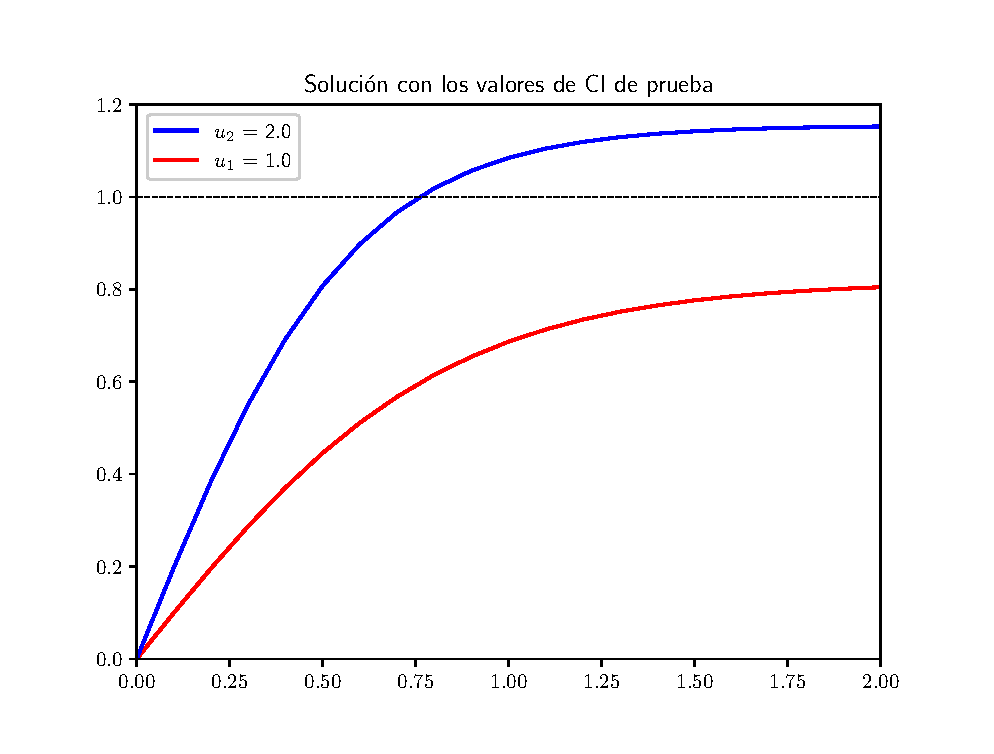
\includegraphics[scale=0.55]{Imagenes/plot_Ejercicio_01_Metodo_Disparo_01.eps}
\end{figure}
\end{frame}
\begin{frame}
\frametitle{Intepretación}
De la figura anterior vemos que los valores de prueba $u_{1} = 1$ y $u_{2} = 2$ quedan por debajo y por arriba, respectivamente, de la solución esperada.
\end{frame}
\begin{frame}
\frametitle{Gráfica con el valor interpolado}
\begin{figure}
    \centering
    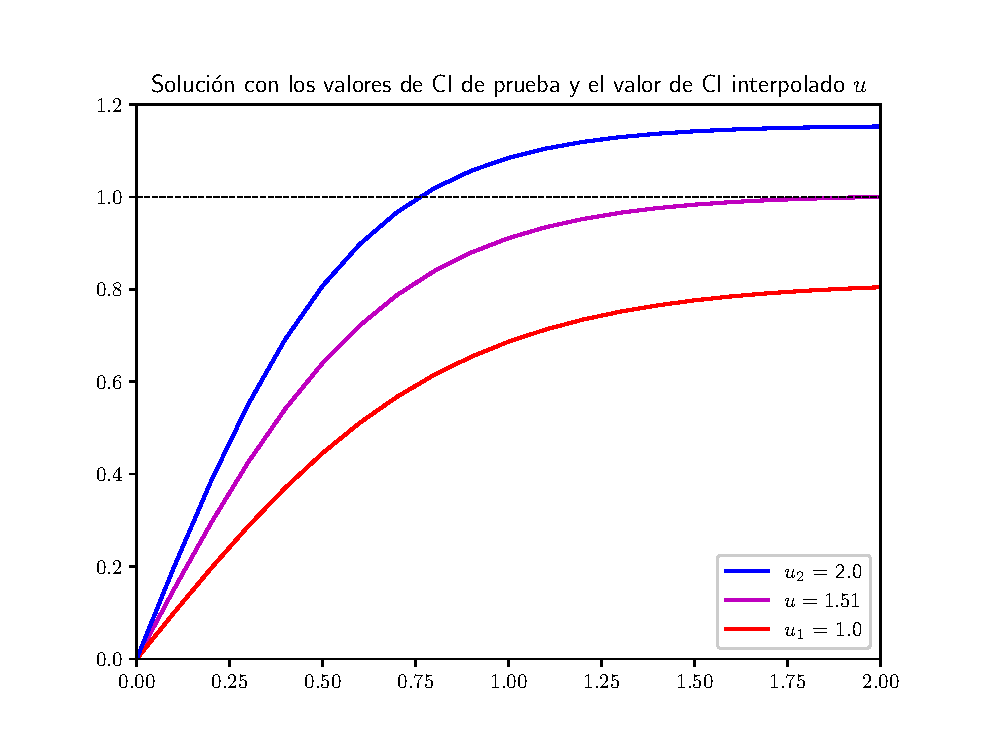
\includegraphics[scale=0.55]{Imagenes/plot_Ejercicio_01_Metodo_Disparo_02.eps}
\end{figure}
\end{frame}
\begin{frame}
\frametitle{Intepretación}
De la figura anterior, ahora vemos que el valor interpolado $u = 1.51$ es con el que se tiene la solución que indica la CDF.
\\
\bigskip
\pause
Esto implica que cada ejercicio deberá de revisarse con cuidado para realizar la prueba y comprobación.
\end{frame}

\subsection{Ejercicio 2}

\begin{frame}
\frametitle{Planteamiento del problema}
Resuelve el siguiente problema de tercer orden con CDF:
\pause
\begin{align*}
\tderivada{y} = 2 \, \sderivada{y} + 6 \, x \, y \hspace{1.3cm} y (0) = 2, \hspace{0.5cm} y (5) = \pderivada{y} (5) = 0
\end{align*}
Una vez resuelto el problema, elabora una gráfica de $y$, $\pderivada{y}$ contra $x$.
\end{frame}
\begin{frame}
\frametitle{Sistema de EDO1}
Nuestro sistema de EDO1 es:
\pause
\begin{align*}
\pderivada{\mathbf{y}} = \begin{bmatrix}
\pderivada{y}_{0} \\
\pderivada{y}_{1} \\
\pderivada{y}_{2}
\end{bmatrix}
&=
\begin{bmatrix}
y_{1} \\
y_{2} \\
2 \, y_{2} + 6 \, x \, y_{0}
\end{bmatrix}
\\
y_{0} &= 2 \hspace{1cm} y_{0} (5) = y_{1} (5) = 0
\end{align*}
\end{frame}
\begin{frame}
\frametitle{Solución al Ejercicio 2}
Como dos de las tres CDF se especifican en el extremo derecho, comenzamos la integración en $x = 5$ y procedemos con un valor de $h$ negativo hacia $x = 0$.
\end{frame}
\begin{frame}
\frametitle{Solución al Ejercicio 2}
Se presentan dos de las tres condiciones iniciales: $y_{0} (5) = y_{1} (5) = 0$, \pause mientras que la tercera condición $y_{2} (5)$ es desconocida.
\\
\bigskip
\pause
Dado que la ED es lineal, reemplazamos la función \funcionazul{ridder} con \funcionazul{interpLin}.
\end{frame}
\begin{frame}
\frametitle{Solución al Ejercicio 2}
En la interpolación lineal, los valores de prueba para $y_{2} (5)$ ($u_{1}$ y $u_{2}$) no son importantes.
\\
\bigskip
Por lo que dejamos los que estaban en el ejemplo anterior. \pause Para la integración se eligió el método adaptativo de Runge-Kutta: \funcionazul{integra\_RKAdaptativo}.
\end{frame}
\begin{frame}
\frametitle{Código para resolver el Ejercicio 2}
El siguiente código implementa la solución para el problema, calculando la solución para las condiciones $u_{1}$ y $u_{2}$, para luego usar el valor de $u$ interpolado.
\end{frame}
\begin{frame}[allowframebreaks, fragile]
\frametitle{Escribiendo las funciones}
\begin{lstlisting}[caption=Las funciones necesarias para el problema]
def interpLineal(f, x1, x2):
    f1 = f(x1)
    f2 = f(x2)

    return x2 - f2 * (x2 - x1) / (f2 - f1)

def condIni(u):
    return np.array([0.0, 0.0, u])

def r(u):
    X, Y = integra_RKAdaptativo(F, xInicio, condIni(u), xAlto, h)
    y = Y[len(Y) - 1]
    r = y[0] - 2.0
    
    return r

def F(x, y):
    F = np.zeros(3)
    F[0] = y[1]
    F[1] = y[2]
    F[2] = 2.0 * y[2] + 6.0 * x * y[0]
    
    return F
\end{lstlisting}
\end{frame}
\begin{frame}[fragile]
\frametitle{Condiciones para el Ejercicio 2}
\begin{lstlisting}[caption=Las condiciones para el ejercicio]
xInicio = 5.0
xAlto = 0.0
u1 = 1.0
u2 = 2.0

h = -0.1
\end{lstlisting}
\end{frame}
\begin{frame}[fragile]
\frametitle{Resolviendo para los $u_{1}$ y $u_{2}$}
\begin{lstlisting}[caption=Evaluando con los valores de prueba]
# Primer intento de CI desconocida
u1 = 1.0
X1, Y1 = integra_RKAdaptativo(F, xInicio, condIni(u1), xAlto, h)

# Primer intento de CI desconocida
u2 = 2.0
X2, Y2 = integra_RKAdaptativo(F, xInicio, condIni(u2), xAlto, h)
\end{lstlisting}
\end{frame}
\begin{frame}[fragile]
\frametitle{Calculando el valor de $u$}
\begin{lstlisting}[caption=Calculando el valor interpolado de u]
# Valor de CI interpolada
u = interpLineal(r, u1, u2)

X3, Y3 = integra_RKAdaptativo(F, xInicio, condIni(u), xAlto, h)    
\end{lstlisting}
\end{frame}
\begin{frame}
\frametitle{Rutina de graficación}
Hay que incluir la correspondiente rutina de graficación en el código.
\end{frame}
\begin{frame}
\frametitle{Gráfica para la primera evaluación}
\begin{figure}
    \centering
    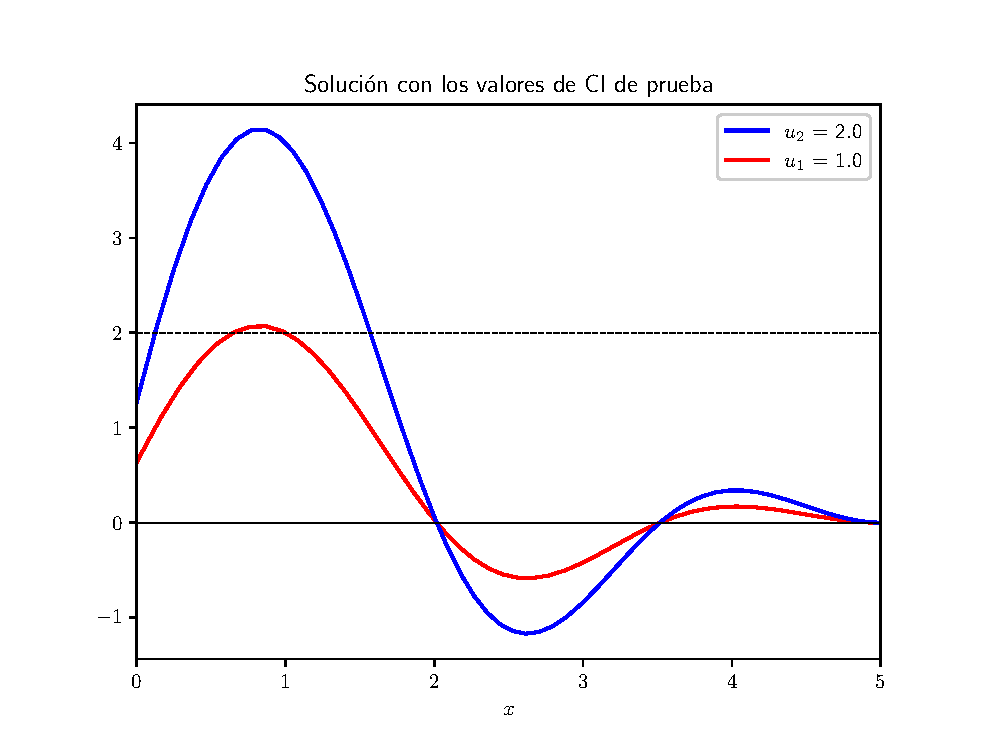
\includegraphics[scale=0.55]{Imagenes/plot_Ejercicio_02_Metodo_Disparo_01.eps}
\end{figure}
\end{frame}
\begin{frame}
\frametitle{Gráfica para la segunda evaluación}
\begin{figure}
    \centering
    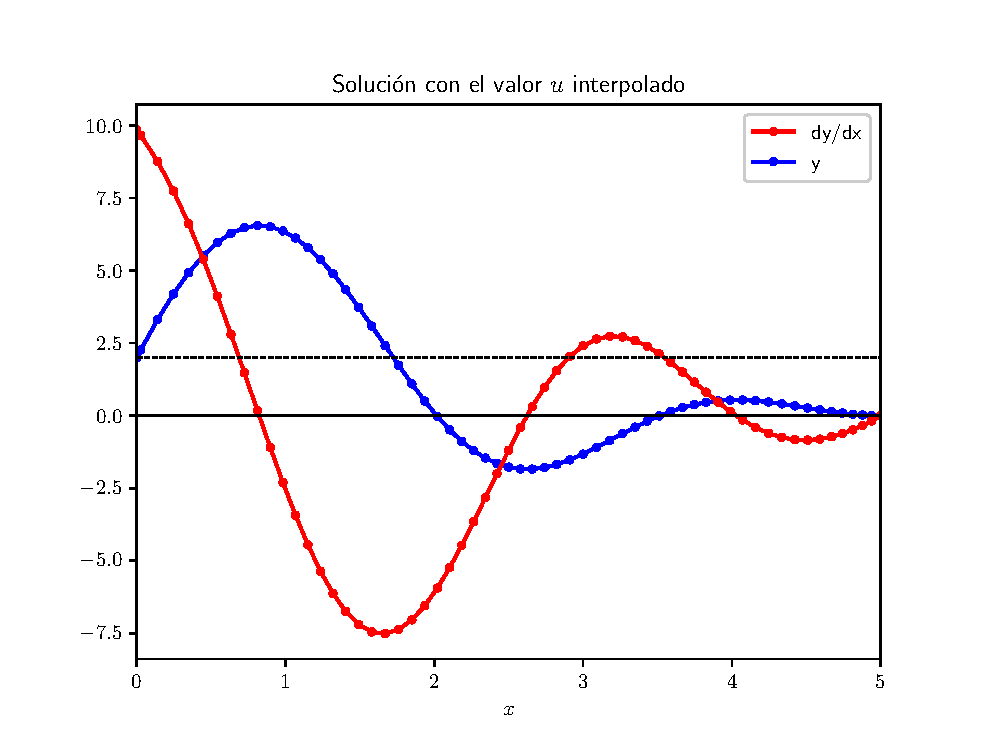
\includegraphics[scale=0.55]{Imagenes/plot_Ejercicio_02_Metodo_Disparo_02.eps}
\end{figure}
\end{frame}

\subsection{Ejercicios a cuenta}

\begin{frame}
\frametitle{Ejercicio a cuenta 1}
Resuelve el siguiente problema con CDF:
\begin{align*}
\sderivada{y} + (1 - 0.2 \, x) \, y^{2} = 0 \hspace{1.3cm} y (0) = 0 \hspace{0.5cm} y \left( \dfrac{\pi}{2} \right) = 1
\end{align*}
\end{frame}
\begin{frame}
\frametitle{Ejercicio a cuenta 2}
Resuelve el siguiente problema con CDF:
\begin{align*}
\sderivada{y} + \sin y + 1 = 0 \hspace{1.3cm} y (0) = 0 \hspace{0.5cm} y (\pi) = 0
\end{align*}
\end{frame}
\begin{frame}
\frametitle{Ejercicio a cuenta 3}
Resuelve el siguiente problema con CDF:
\begin{align*}
\tderivada{y} + 2 \, \sderivada{y} + \sin y = 0 \\
y (-1) = 0 \hspace{0.5cm} \pderivada{y} (-1) = -1 \hspace{0.5cm} \pderivada{y} (1) = 1
\end{align*}
\end{frame}

\section{Método de diferencias finitas}
\frame{\tableofcontents[currentsection, hideothersubsections]}
\subsection{Definición}

\begin{frame}
\frametitle{El método de diferencias finitas}
En el \textbf{\textcolor{burgundy}{método de diferencias finitas}}, se divide el intervalo de integración $(a, b)$ en $m$ subintervalos iguales de longitud $h$ cada uno.

\end{frame}
\begin{frame}
\frametitle{Identificando los puntos}
Los valores de la solución numérica en los puntos de la \textbf{\textcolor{cadmiumgreen}{malla}} se indican mediante $y_{i}$, donde $i = 0, 1, \ldots, m$.
\end{frame}
\begin{frame}
\frametitle{Identificando los puntos}
\begin{figure}
\centering
\begin{tikzpicture}[font=\scriptsize]
    \draw (0, 0) -- (8, 0) node [above, near end, pos=1] {$x$};
    \draw (0, 0) -- (0, 4) node [left, near end, pos=1.1] {$y$};
    \draw (1, 1) .. controls (2, 2.5) and (5.5, 3.5) .. (6.5, 3.5);
    \draw [dashed] (0.5, 0.4) -- (1, 1);
    \draw [dashed] (6.5, 3.5) -- (7, 3.3);

    \node at (0.5, -0.3) {$x_{-1}$};
    \node at (1, -0.3) {$x_{0}$};
    \node at (1, -0.8) {$a$};

    \node at (1.5, -0.3) {$x_{1}$};
    \node at (2, -0.3) {$x_{2}$};
    \node at (2.5, -0.3) {$x_{3}$};

    \draw [dashed] (0.5, 0) -- (0.5, 0.4) node [midway, right] {$y_{-1}$};
    \draw [dashed] (1, 0) -- (1, 1) node [midway, right] {$y_{0}$};
    \draw [dashed] (1.5, 0) -- (1.5, 1.5) node [midway, right] {$y_{1}$};
    \draw [dashed] (2, 0) -- (2, 1.95) node [midway, right] {$y_{2}$};
    \draw [dashed] (2.5, 0) -- (2.5, 2.3) node [midway, right] {$y_{3}$};

    \draw [<->] (2, 0.3) -- (2.5, 0.3) node[above, midway] {$h$};

    \draw (1, 1) circle (1pt);
    \draw (1.5, 1.55) circle (1pt);
    \draw (2, 1.92) circle (1pt);
    \draw (2.5, 2.24) circle (1pt);

    
    \node at (6, -0.6) {$x_{m\!-1}$};
    \node at (6.5, -0.3) {$x_{m}$};
    \node at (6.5, -0.8) {$b$};

    \node at (7, -0.6) {$x_{m\!+1}$};

    \draw (6, 3.45) circle (1pt);
    \draw (6.5, 3.46) circle (1pt);

    \draw [dashed] (6, 0) -- (6, 3.4);
    \draw [dashed] (6.5, 0) -- (6.5, 3.45);
    \draw [dashed] (7, 0) -- (7, 3.3);

    \node at (5.8, 2) [rotate=90] {$y_{m-1}$};
    \node at (6.3, 2) [rotate=90] {$y_{m}$};
    \node at (6.8, 2) [rotate=90] {$y_{m+1}$};
\end{tikzpicture}
\end{figure}
El propósito de $y_{-1} $ e $y_{m+1}$ se explicará en breve.
\end{frame}
\begin{frame}
\frametitle{Las aproximaciones}
Ahora hacemos dos aproximaciones:
\pause
\\
\bigskip
\pause
\setbeamercolor{item projected}{bg=capri,fg=black}
\setbeamertemplate{enumerate items}{%
\usebeamercolor[bg]{item projected}%
\raisebox{1.5pt}{\colorbox{bg}{\color{fg}\footnotesize\insertenumlabel}}%
}
\begin{enumerate}
\item Las derivadas de $y$ en la ED se reemplazan por las expresiones en diferencias finitas. Es una práctica común utilizar las aproximaciones en primeras diferencias centrales (como lo vimos en el Tema 2):
\begin{align}
\pderivada{y}_{i} = \dfrac{y_{i+1} - y_{i-1}}{2 \, h} \hspace{1.5cm} \sderivada{y}_{i} = \dfrac{y_{i-1} - 2 \, y_{i} +  y_{i+1}}{h^{2}} \hspace{0.5cm} \text{etc.}
\end{align}
\seti
\end{enumerate}
\end{frame}
\begin{frame}
\frametitle{Las aproximaciones}
\setbeamercolor{item projected}{bg=capri,fg=black}
\setbeamertemplate{enumerate items}{%
\usebeamercolor[bg]{item projected}%
\raisebox{1.5pt}{\colorbox{bg}{\color{fg}\footnotesize\insertenumlabel}}%
}
\begin{enumerate}[<+->]
\item La ecuación diferencial se aplica solo en los puntos de malla.
\end{enumerate}
\end{frame}
\begin{frame}
\frametitle{El resultado}
Como resultado, las ED se reemplazan por $m + 1$ \textbf{\textcolor{chestnut}{ecuaciones algebraicas simultáneas}}, \pause siendo las incógnitas $y_{i}$ donde $i = 0, 1, \ldots, m$.
\\
\bigskip
Si la ED es no lineal, las ecuaciones algebraicas también serán no lineales y deberán resolverse por el método de Newton-Raphson.
\end{frame}
\begin{frame}
\frametitle{El error asociado}
Dado que el error de truncamiento en una aproximación en primera diferencia central es $\order{h^{2}}$, \pause el método de diferencias finitas no es tan preciso como el método de disparo.
\end{frame}
\begin{frame}
\frametitle{El error asociado}
Recordemos que el método de Runge-Kutta tiene un error de truncamiento de $\order{h^{5}}$.
\\
\bigskip
\pause
Por lo tanto, el criterio de convergencia especificado en el método de Newton-Raphson no debería ser demasiado severo.
\end{frame}

\subsection{Una ED2}

\begin{frame}
\frametitle{Desarrollando el método}
Considera la siguiente ED2:
\pause
\begin{align*}
\sderivada{y} = f (x, y, \pderivada{y})
\end{align*}
\pause
con las CDF:
\begin{align*}
y (a) &= \alpha \hspace{0.5cm} \text{o} \hspace{0.5cm} \pderivada{y} (a) = \alpha \\
y (b) &= \beta \hspace{0.5cm} \text{o} \hspace{0.5cm} \pderivada{y} (b) = \beta
\end{align*}
\end{frame}
\begin{frame}
\frametitle{Evaluando las derivadas}
Aproximando las derivadas en los puntos de malla por diferencias finitas, el problema se convierte en:
\pause
\begin{eqnarray}
\dfrac{y_{i-1} - 2 \, y_{i} +  y_{i+1}}{h^{2}} &=& f \bigg( x_{i}, y_{i}, \dfrac{y_{i+1} - y_{i-1}}{2 \, h} \bigg) \label{eq:ecuacion_08_09} \\ \pause
y_{0} &=& \alpha \hspace{0.5cm} \text{o} \hspace{0.5cm} \dfrac{y_{1} - y_{-1}}{2 \, h} = \alpha \label{eq:ecuacion_08_10a} \\ \pause
y_{m} &=& \beta \hspace{0.5cm} \text{o} \hspace{0.5cm} \dfrac{y_{m+1} - y_{m-1}}{2 \, h} = \beta \label{eq:ecuacion_08_10b}
\end{eqnarray}
\end{frame}
\begin{frame}
\frametitle{De los valores antes y después de la malla}
Tengamos en cuenta la presencia tanto de $y_{-1}$ como de $y_{m+1}$, \pause que están asociados con puntos fuera del dominio de la solución $(a,b)$.
\\
\bigskip
\pause
Este \enquote{exceso} se puede eliminar utilizando las CDF.
\end{frame}
\begin{frame}
\frametitle{Reescribiendo la ecuación}
Pero antes de hacer eso, reescribamos las ecs. (\ref{eq:ecuacion_08_09}) como:
\pause
\begin{eqnarray}
&{}& y_{-1} - 2 \, y_{0} + y_{1} - h^{2}  f \bigg( x_{0}, y_{0}, \dfrac{y_{1} - y_{-1}}{2 \, h} \bigg) = 0 \label{eq:ecuacion_a} \\ \pause
&{}&y_{i-1} - 2 \, y_{i} + y_{i+1} - h^{2}  f \bigg( x_{i}, y_{i}, \dfrac{y_{i+1} - y_{i-1}}{2 \, h} \bigg) = 0 \label{eq:ecuacion_b}\\
&i& = 1, 2, \ldots, m-1 \nonumber \\ \pause
&{}& y_{m-1} - 2 \, y_{m} + y_{m+1} + \nonumber \\
&{}& - h^{2} \, f \bigg( x_{m}, y_{m}, \dfrac{y_{m+1} - y_{m-1}}{2 \, h} \bigg) = 0 \label{eq:ecuacion_c}
\end{eqnarray}
\end{frame}
\begin{frame}
\frametitle{De las CDF}
Las CDF en $y$ se tratan fácilmente:
\pause
\setbeamercolor{item projected}{bg=coralred,fg=white}
\setbeamertemplate{enumerate items}{%
\usebeamercolor[bg]{item projected}%
\raisebox{1.5pt}{\colorbox{bg}{\color{fg}\footnotesize\insertenumlabel}}%
}
\begin{enumerate}[<+->]
\item La ec. (\ref{eq:ecuacion_a}) simplemente se reemplaza por $y_{0} - \alpha = 0$.
\item La ec. (\ref{eq:ecuacion_c}) se reemplaza por $y_{m} - \beta = 0$.
\end{enumerate}
\end{frame}
\begin{frame}
\frametitle{Valores proporcionados}
Si se indica $\pderivada{y}$, obtenemos de las ecs. (\ref{eq:ecuacion_08_10a} - \ref{eq:ecuacion_08_10b}):
\pause
\begin{align*}
y_{-1} = y_{1} - 2 \, h \, \alpha \\
y_{m+1} = y_{m-1} + 2 \, h \, \beta
\end{align*}
\pause
que luego se sustituyen en las ecs. (\ref{eq:ecuacion_a}) y (\ref{eq:ecuacion_c}), respectivamente.
\end{frame}
\begin{frame}
\frametitle{Sistema resultante}
Por lo tanto, terminamos con $m + 1$ ecuaciones en las incógnitas $y_{0}, y_{1}, \ldots, y_{m}$:
\pause
\begin{eqnarray}
\begin{aligned}
&y_{0} - \alpha = 0 \hspace{1cm} \text{si } y (a) = \alpha \\
&-2 \, y_{0} + 2 \, y_{1} - h^{2} \, f (x_{0}, y_{0}, \alpha) - 2\, h \, \alpha = 0 \hspace{1cm} \text{si } \pderivada{y} (a) = \alpha \\
\end{aligned}
\label{eq:ecuacion_08_11_a}
\end{eqnarray}
\end{frame}
\begin{frame}
\frametitle{Sistema resultante}
\begin{align}
&{}y_{i-1} - 2 \, y_{i} + y_{i+1} - h^{2}  f \bigg( x_{i}, y_{i}, \dfrac{y_{i+1} - y_{i-1}}{2 \, h} \bigg) = 0 \label{eq:ecuacion_08_11_b}\\
&{}i = 1, 2, \ldots, m-1 \nonumber
\end{align}
\end{frame}
\begin{frame}
\frametitle{Sistema resultante}
\begin{eqnarray}
\begin{aligned}
&y_{m} - \beta = 0 \hspace{1cm} \text{si } y (b) = \beta \\
&-2 \, y_{m-1} + 2 \, y_{m} - h^{2} \, f (x_{m}, y_{m}, \beta) - 2 \, h \, \beta = 0 \\
&\text{si } \pderivada{y} (b) = \beta
\end{aligned}
\label{eq:ecuacion_08_11_c}
\end{eqnarray}
\end{frame}
% \begin{frame}
% \frametitle{Problemas con CDF y valores propios}
% Otra tipo de problemas de la física requiere la solución de ED con valores de las magnitudes físicas o sus derivadas en las fronteras de una región.
% \\
% \medskip
% \pause
% Por ejemplo:
% \begin{itemize}[<+->]
% \item La solución de la ecuación de Poisson con una distribución de carga dada y valores conocidos de potencial electrostático en la frontera.
% \item La ecuación de Schrödinger estacionaria con un potencial dado y condiciones de frontera.
% \end{itemize}
% \end{frame}
% \begin{frame}
% \frametitle{EDO con CDF}
% Un problema de típico con \textbf{\textcolor{carmine}{condiciones de frontera en física}}, por lo general se presenta en forma de una ecuación diferencial de segundo orden:
% \begin{align}
% \sderivada{u} = f( u, \pderivada{u}; x)
% \label{eq:ecuacion1}
% \end{align} 
% donde $u$ es una función de $x$; $\pderivada{u}$ y $\sderivada{u}$ son las derivadas de primer y segundo orden de $u$ con respecto a $x$, $f(u, \pderivada{u}; x)$ es una función de $u$, $\pderivada{u}$ y $x$. Por lo que $u$ o $\pderivada{u}$ están dadas como puntos en la frontera.
% \end{frame}
% \begin{frame}
% Considera que sin pérdida de generalidad, siempre podemos elegir un sistema coordenado tal que las fronteras del sistema sean $x=0$ y $x=1$, siempre y cuando el sistema sea finito.
% \\
% \medskip
% Por ejemplo, para un problema dado si el sistema tiene las fronteras en $x=x_{1}$ y $x=x_{2}$, siempre podemos hacer $x'=0$ y $x'=1$ con una transformación
% \begin{equation}
% x' = \dfrac{x-x_{1}}{x_{2} - x_{1}}
% \end{equation} 
% \end{frame}
% \begin{frame}
% Para problemas de una dimensión, tenemos un total de cuatro tipo de condiciones de frontera:
% \begin{enumerate}
% \item $u(0) = u_{0}$ y $u(1) = u_{1}$ 
% \item $u(0) = u_{0}$ y $u'(1) = v_{1}$
% \item $u'(0) = v_{0}$ y $u(1) = u_{1}$
% \item $u'(0) = v_{0}$ y $u'(1) = v_{1}$   
% \end{enumerate}
% \end{frame}
% \begin{frame}
% Un problema de valores en la frontera es más difícil de resolver que un problema de valores iniciales.
% \\
% \medskip
% Si queremos resolver un problema de valores iniciales del tipo de la ecuación (\ref{eq:ecuacion1}), donde re-emplazamos $x$ por $t$ y las condiciones iniciales $u(0) = u_{0}$ y $u'(0) = v_{0}$, podemos transformar la ED en un conjunto de dos EDO-1, como lo hemos venido haciendo.
% \\
% \medskip
% Sin embargo, para el problema de valores en la frontera (VEF), sólo conocemos $u(0)$ o $u'(0)$, que no es lo suficiente para utilizar alguno de los algoritmos que conocemos para las EDO-1 de valores iniciales (Taylor, Euler, RK4)
% \end{frame}
% \section{Problemas de valores propios}
% \begin{frame}
% \frametitle{Problemas de valores propios}
% Los problemas típicos de valores propios son aún más complicados, ya que al menos un parámetro más, el \emph{valor propio}, está involucrado en la ecuación, por ejemplo:
% \begin{equation}
% u'' = f(u, u'; x; \lambda)
% \label{eq:ecuacion_vp}
% \end{equation}
% junto con un conjunto de condiciones de frontera, definen un problema de valores propios.
% \\
% \medskip
% El valor propio $\lambda$(también llamado \emph{eigenvalor}), puede tener sólo algunos valores determinados  con el fin de proporcionar soluciones aceptables de la ecuación, con las condiciones de frontera establecidas.
% \end{frame}
% \begin{frame}
% \frametitle{Ejemplo}
% Consideremos las vibraciones longitudinales a lo largo de una cuerda elástica, la ecuación que describe la solución estacionaria de las ondas elásticas es
% \begin{equation}
% u''(x) = - k^{2} u(x)
% \end{equation}
% donde $u(x)$ es el desplazamiento sobre el punto de equilibrio $x$ y los valores permitidos de $k^{2}$ son los valores propios del problema.
% \\
% \medskip
% El vector de onda $k$ en la ecuación, está relacionado con la velocidad de fase $c$ de la onda a lo largo de la cuerda, y la frecuencia angular $\omega$ permitida, por la relación
% \begin{equation}
% \omega = ck
% \end{equation}
% \end{frame}
% \begin{frame}
% Si los extremos de la cuerda están fijos ($x=0$ y $x=1$), las condiciones de frontera son por tanto: $u(0)=u(1)=0$. Si un extremo de la cuerda ($x=0$) está fijo y el otro libre ($x=1$), las condiciones de frontera ahora son $u(0)=0$ y $u'(0)=1$. Para este problema, podemos obtener una solución analítica.
% \\
% \medskip
% Por ejemplo, si los extremos de la cuerda están fijos, las funciones propias
% \begin{equation}
% u_{l}(x) = \sqrt{2} \sin k_{l} x
% \end{equation}
% son las posibles soluciones de la ED.
% \\
% \medskip
% \pause
% Los valores propios están dados por
% \begin{equation}
% k_{l}^{2} = (l \pi)^{2}
% \end{equation}
% con $l=1,2,\ldots,\infty$. 
% \end{frame}
% \begin{frame}
% La solución completa de las ondas a lo largo de la cuerda elástica están dadas por una combinación lineal de las funciones propias con las soluciones de valores iniciales, en este caso
% \begin{equation}
% u(x,t) = \sum_{l=1}^{\infty} (a_{l} \sin \omega_{l} t + b_{i} \cos \omega_{l} t) u_{l}(x)
% \end{equation}
% donde $\omega_{l} = c k_{l}$, $a_{l}$ y $b_{l}$ son los coeficientes determinados por las condiciones iniciales.
% \end{frame}
% \section{Método de disparo}
% \begin{frame}
% \frametitle{Método de disparo}
% Un método sencillo para resolver problemas de ED-CVF (ecuación \ref{eq:ecuacion1}) y los problemas de valores propios (ecuación \ref{eq:ecuacion_vp}), es el llamado \emph{método de disparo}.
% \\
% \medskip
% Veamos cómo funciona para problemas CVF y luego, generalizar para problemas de valores propios.
% \end{frame}
% \begin{frame}
% Como hemos hecho en el caso de tener un problema de una ED de orden 2, hacemos un cambio de variable, para dejar un sistema de EDO-1, haciendo $y_{1}=u$ y $y_{2}=u'$, por tanto
% \begin{eqnarray}
% \dfrac{dy_{1}}{dx} &=& y_{2} \\
% \dfrac{dy_{2}}{dx} &=& f(y_{1}, y_{2}; x)
% \end{eqnarray}
% suponiendo las siguientes CVF $u(0)= u_{0}$ y $u(1)= u_{1}$. Para otro tipo de problemas con otras CVF, se pueden resolver de manera similar.
% \end{frame}
% \begin{frame}
% El punto importante es hacer que el problema se parezca a un problema de valores iniciales, utilizando un parámetro que se ajuste, por lo que la solución se obtiene al variar el parámetro.
% \\
% \medskip
% Como $u(0)$ ya está dado, podemos hacer una estimación para la derivada de primer orden en $x=0$, por ejemplo, $u'(0)=\alpha$. Donde $\alpha$ es el parámetro que estará variando.
% \\
% \medskip
% \pause
% Para un valor específico de $\alpha$, podemos integrar la ecuación para $x=1$ con alguna de las técnicas que hemos visto para EDO-1.
% \end{frame}
% \begin{frame}
% Considerando que la elección inicial de  $\alpha$ difícilmente pudiese ser la derivada en $x = 0$, el valor de la función $u_{\alpha} (1)$, resultante de la integración con $u'(0) = \alpha$  para $x = 1$, podría no ser el mismo que $u_{1}$.
% \\
% \medskip
% La idea del método de disparo es utilizar alguno de los algoritmos de búsqueda de la raíz para encontrar la $\alpha$ apropiada, que asegure $f(\alpha) = u_{\alpha} (1) - u_{1} = 0$, con una tolerancia $\delta$ dada.
% \end{frame}
% \begin{frame}
% \frametitle{Ejemplo}
% Hagamos un ejercicio para revisar el método. Sea la siguiente EDO-2
% \begin{equation}
% u'' = - \dfrac{\pi^{2}}{4}(u+1)
% \end{equation}
% y las CVF son $u(0)=0$ y $u(1)=1$. 
% \\
% \medskip
% \pause
% Definimos $y_{1}=u$ y $y_{2}=u'$, por lo que tenemos ahora
% \begin{eqnarray}
% \dfrac{dy_{1}}{dx} &=& y_{2} \\
% \dfrac{dy_{2}}{dx} &=& - \dfrac{\pi^{2}}{4}(y_{1} + 1)
% \end{eqnarray}
% \end{frame}
% \begin{frame}
% Asumimos que la ecuación tiene los valores iniciales $y_{1}(0)=0$ y $y_{2}(0) = \alpha$.
% \\
% \medskip
% \pause
% El valor de $\alpha$ tendrá que ajustarse para que $f(\alpha) = u_{\alpha}(1) - 1 = 0$.
% \\
% \medskip
% Podemos combinar el método de la secante y resolver el sistema de EDO-1 como lo hemos venido haciendo.
% \\
% \medskip
% Resuelve y grafica el problema usando primero un valor de $\alpha=1.0$ y luego con $\alpha=4.0$. El problema cuenta para el Tema 3 y se considera resuelto cuando proporcionas el valor de $\alpha$ con el cual se cumplen las CVF y su respectiva gráfica.
% \end{frame}
% \begin{frame}[fragile]
% \frametitle{Solución con $y0 = array([0.0,\alpha=1.0])$}
% \begin{figure}
% 	\centering
% 	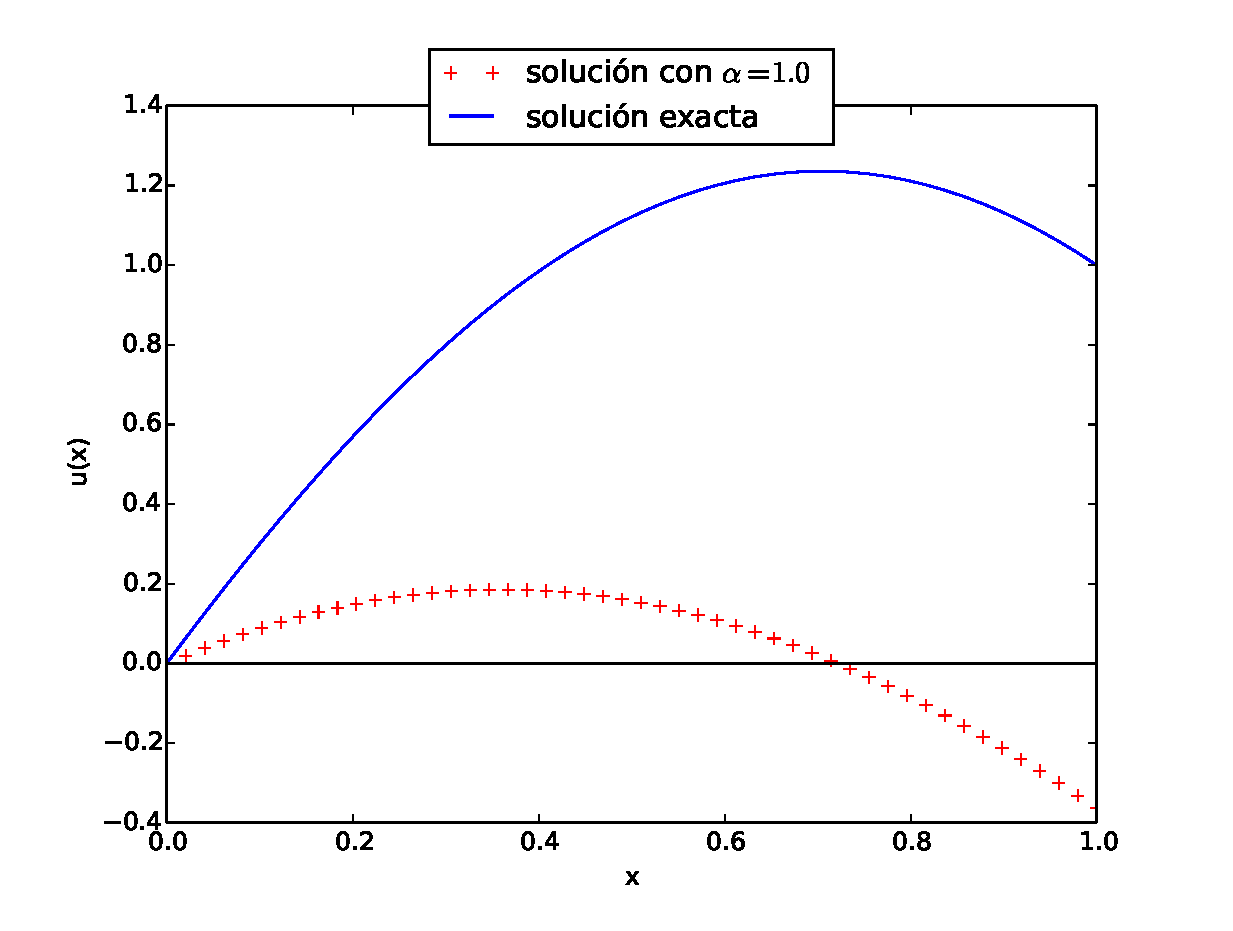
\includegraphics[scale=0.5]{MetodoDisparo2014_01.eps}
% \end{figure}
% \end{frame}
% \begin{frame}[fragile]
% \frametitle{Solución con $y0 = array([0.0,\alpha=4.0])$}
% \begin{figure}
% 	\centering
% 	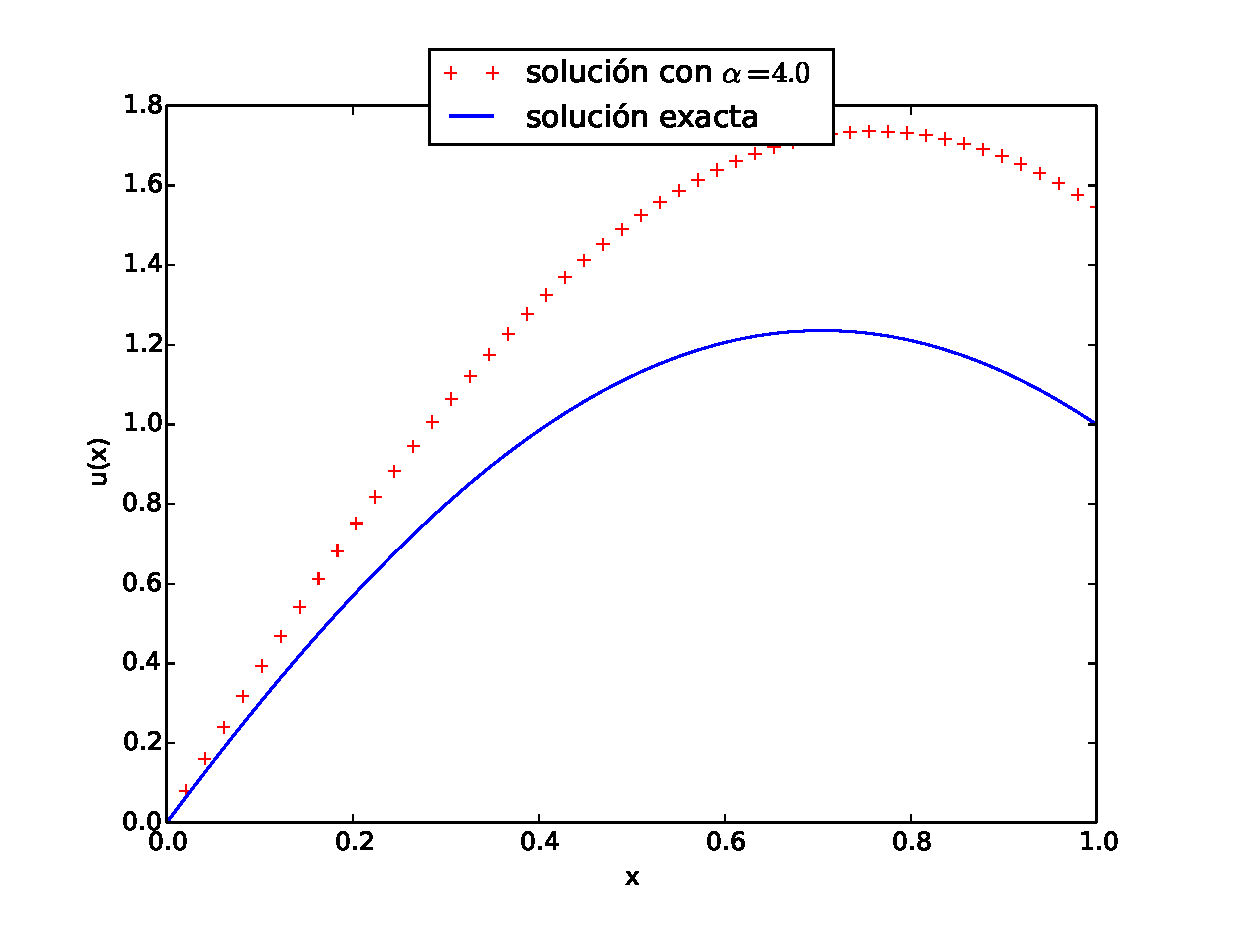
\includegraphics[scale=0.5]{MetodoDisparo2014_02.eps}
% \end{figure}
% \end{frame}
% \begin{frame}
% \frametitle{¿Qué hacemos?}
% El siguiente paso es encontrar el valor de la raíz en donde $f(\alpha) = u_{\alpha}(1) - 1 = 0$.
% \\
% \medskip

% Revisando los valores que obtenemos para $\alpha$:
% \\
% \medskip
% $u_{1.0}(1) = -0.3633$ \\
% $u_{4.0}(1) = 1.5464$
% \\
% \medskip
% Por lo que necesariamente hay una raíz que debemos de utilizar para sustituirla en nuestro problema.
% \end{frame}
% \begin{frame}
% El problema CVF se resuelve de manera exacta, la solución analítica es:
% \begin{equation}
% u(x) = \cos\left(\frac{x \pi}{2}\right) + 2 \sin \left(\frac{x \pi}{2}\right) -1
% \end{equation}
% \end{frame}
% \begin{frame}
% \frametitle{Pasos a realizar}
% \begin{enumerate}
% \item Construir una tabla de valores $\alpha$ y $f(\alpha) = u_{\alpha}(1) - 1$.
% \item Usando el método de la secante, obtener el valor de la raíz tal que $f(\alpha)=0$. El método de la secante que construimos en el Tema 2, requiere de dos valores iniciales, para esa función, dabamos una función $f$ que python evalúa al momento, ahora nuestra función es una tabla de pares ordenados $\alpha$ y $f(\alpha)$, por lo que hay que ajustar nuestro código para que reciba esos valores y nos devuelva la raíz.
% \item El valor de la raíz, lo usamos como argumento en $y0=[0.0, \alpha]$ y resolvemos la ecuación diferencial.
% \end{enumerate}
% \end{frame}
% \begin{frame}[fragile]
% \frametitle{Solución con $y0 = array([0.0,\alpha=??])$}
% \begin{figure}
% 	\centering
% 	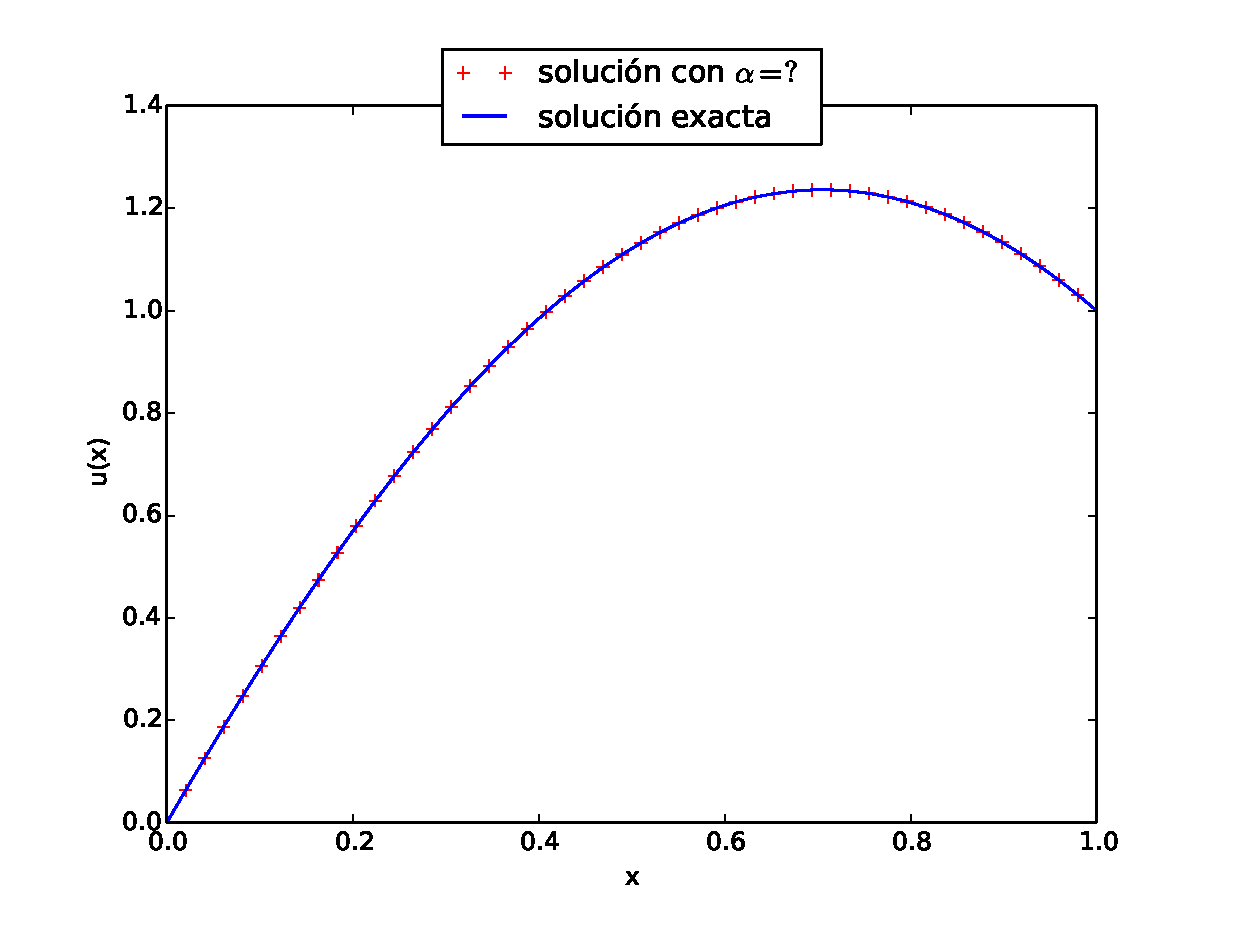
\includegraphics[scale=0.5]{MetodoDisparo2014_03.eps}
% \end{figure}
% \end{frame}
% \begin{frame}
% Problemas con otros tipos de CVF se pueden resolver de manera similar. Por ejemplo:
% \\
% \medskip
% si $u'(0)=v_{0}$ y $u(1)=u_{1}$ están dados, podemos hacer una estimación de $u(0)=\alpha$ e integrar el conjunto de ecuaciones de $y_{1}$ y $y_{2}$ en $x=1$. La raíz a buscar está en $f(\alpha) = u_{\alpha}(1) - u_{1} = 0$. Aquí el valor de $u_{\alpha}(1)$ es el resultado de la ecuación con $u(0)=\alpha$.
% \end{frame}
% \begin{frame}
% Cuando se aplica el método de disparo para los problemas de valores propios, el parámetro a ajustar no es mayor que el valor propio del problema.
% \\
% \medskip
% Por ejemplo, si están dados $u(0)=u_{0}$ y $u(1)=u_{1}$, podemos integrar la ecuación con $u'(0)= \alpha$, que es un valor pequeño. Luego, buscamos la raíz de $f(\lambda) = u_{\lambda}(1) - u_{1}=0$ variando $\lambda$.
% \\
% \medskip
% Cuando $f(\lambda)=0$ se satisface, obtenemos un valor propio aproximado $\lambda$ y el correspondiente estado propio de la solución normalizada de $u_{\lambda}(x)$.
% \end{frame}
%\section{EDO con valores en las fronteras}
%\begin{frame}
%\frametitle{EDO con valores en las fronteras}
%En lo que hemos visto del tema, recordamos que una EDO se acompaña de condiciones auxiliares. Estas condiciones se usan para evaluar las constantes de integración que resultan durante la solución de la ecuación. 
%\\
%\bigskip
%Para una ecuación de $n$-ésimo orden, se requieren $n$ condiciones. Si todas las condiciones se especifican en el mismo valor de la variable independiente, entonces estamos tratando con un problema de valor inicial.
%\end{frame}
%\begin{frame}
%En contraste, hay un conjunto de problemas en los cuales las condiciones no son conocidas en un solo punto, sino, más bien, son conocidas en diferentes valores de la variable independiente.
%\\
%\bigskip
%Como estos valores se especifican a menudo en los puntos extremos o fronteras de un sistema, se les conoce como problemas de valores en la frontera.
%\end{frame}
%\begin{frame}
%\frametitle{Ejemplo}
%Se puede usar la conservación de calor para desarrollar un balance de calor para una barra larga y delgada. Si la barra no está aislada en toda su longitud y el sistema se encuentra en estado estable, la ecuación resultante es
%\begin{equation} \label{eq:ec_calor1}
% \dfrac{d^{2}T}{dx^{2}} + \alpha(T_{a} - T) = 0 
%\end{equation}
%donde $\alpha$ es un coeficiente de transferencia de calor ($cm^{-2}$) que parametriza la razón de disipación de calor con el aire circundante, y $T_{a}$ es la temperatura del aire circundante.
%\end{frame}
%\begin{frame}
%\frametitle{Problema de temperatura}
%\begin{tikzpicture}[font=\small]
%\draw [pattern=north east lines] (-1,-2) rectangle (0,2);
%\draw (-1,-2) -- node [midway, left] {$T_{1}$}(-1,2);
%\draw (0,-0.5) rectangle (7,0.5);
%\draw [pattern=north east lines] (7,-2) rectangle (8,2);
%\draw (8,-2) -- node [midway, right] {$T_{2}$}(8,2);
%\draw (3.3,1.8) node {$T_{a}$};
%\foreach \x in {1cm, 3cm, 5cm}
%	\draw [->, thick] (\x,0.7) -- (\x,1.3);
%\foreach \x in {1cm, 3cm, 5cm}
%	\draw [->, thick] (\x,-0.8) -- (\x,-1.4);
%\draw [->, thick] (1,0) -- (6,0);
%\draw (-0.1,-2.3) node {x=0};
%\draw (7.1,-2.3) node {x=L};
%\end{tikzpicture}
%\end{frame}
%\begin{frame}
%Para obtener una solución para la ecuación (\ref{eq:ec_calor1}) se deben tener las condiciones en la frontera adecuadas. Un caso simple se presenta donde los valores de las temperaturas en los extremos de la barra se mantienen con valores fijos. Estos valores se pueden
%expresar matemáticamente como
%\[ \begin{split} 
%T_{0} =& T_{1} \\
%T_{L} =& T_{2}
%\end{split} \]
%Con estas condiciones, la ecuación (\ref{eq:ec_calor1}) se puede resolver de manera analítica.
%\end{frame}
%\begin{frame}
%Para una barra de 10 metros con $T_{a} = 20$, $T_{1} = 40$, $T_{2} = 200$ y $\alpha = 0.01$, el resultado es
%\[ T = 73.4523 \exp(0.1x) - 53.4523 \exp (-0.1x) + 20\]
%\end{frame}
%\section{El método de disparo}
%\begin{frame}
%\frametitle{El método de disparo}
%El método de disparo se basa en convertir el problema de valor en la frontera en un problema equivalente de valor inicial.
%\\
%\bigskip
%Posteriormente se implementa un procedimiento de prueba y error para resolver la versión de valor inicial. El procedimiento se puede ilustrar con un ejemplo.
%\end{frame}
%\begin{frame}
%\frametitle{Problema}
%Utilizando el método de disparo para resolver la ecuación (\ref{eq:ec_calor1}), para una barra de 10 metros, con $\alpha= 0.01m^{2}$, $T_{a}=20^{\circ}$C, y las condiciones de frontera
%\[ \begin{split} 
%T(0)=& 40 \\
%T(10) =& 200 
%\end{split} \]
%\end{frame}
%\begin{frame}
%\frametitle{Solución}
%Transformamos la ecuación (\ref{eq:ec_calor1}) en dos EDO de primer orden:
%\begin{eqnarray*}
%\dfrac{dT}{dx} &=& z \\
%\dfrac{dz}{dz} &=& \alpha (T - T_{a})
%\end{eqnarray*}
%Para resolver estas ecuaciones, se requiere un valor inicial para $z$, por el método de disparo, intuimos un valor, digamos $z(0)=10$. Usando RK4 en las dos ecuaciones obtenemos
%\end{frame}
%\begin{frame}
%\fontsize{12}{12}\selectfont
%\begin{center}
%\begin{tabular}{c | c | c}
% x & y[0] & y[1] \\ \hline
%0.0000e+00 & 4.0000e+01 & 1.0000e+01 \\ \hline
%1.0000e+00 & 5.0117e+01 & 1.0250e+01 \\ \hline
%2.0000e+00 & 6.0535e+01 & 1.0603e+01 \\ \hline
%3.0000e+00 & 7.1359e+01 & 1.1062e+01 \\ \hline
%4.0000e+00 & 8.2697e+01 & 1.1632e+01 \\ \hline
%5.0000e+00 & 9.4662e+01 & 1.2318e+01 \\ \hline
%6.0000e+00 & 1.0737e+02 & 1.3128e+01 \\ \hline
%7.0000e+00 & 1.2096e+02 & 1.4069e+01 \\ \hline
%8.0000e+00 & 1.3556e+02 & 1.5151e+01 \\ \hline
%9.0000e+00 & 1.5131e+02 & 1.6384e+01 \\ \hline
%1.0000e+01 & 1.6838e+02 & 1.7781e+01 
%\end{tabular}
%\end{center}
%\end{frame}
%\begin{frame}
%\frametitle{Gráficamente con $Z(0)= 10$}
%\begin{figure}
%	\centering
%	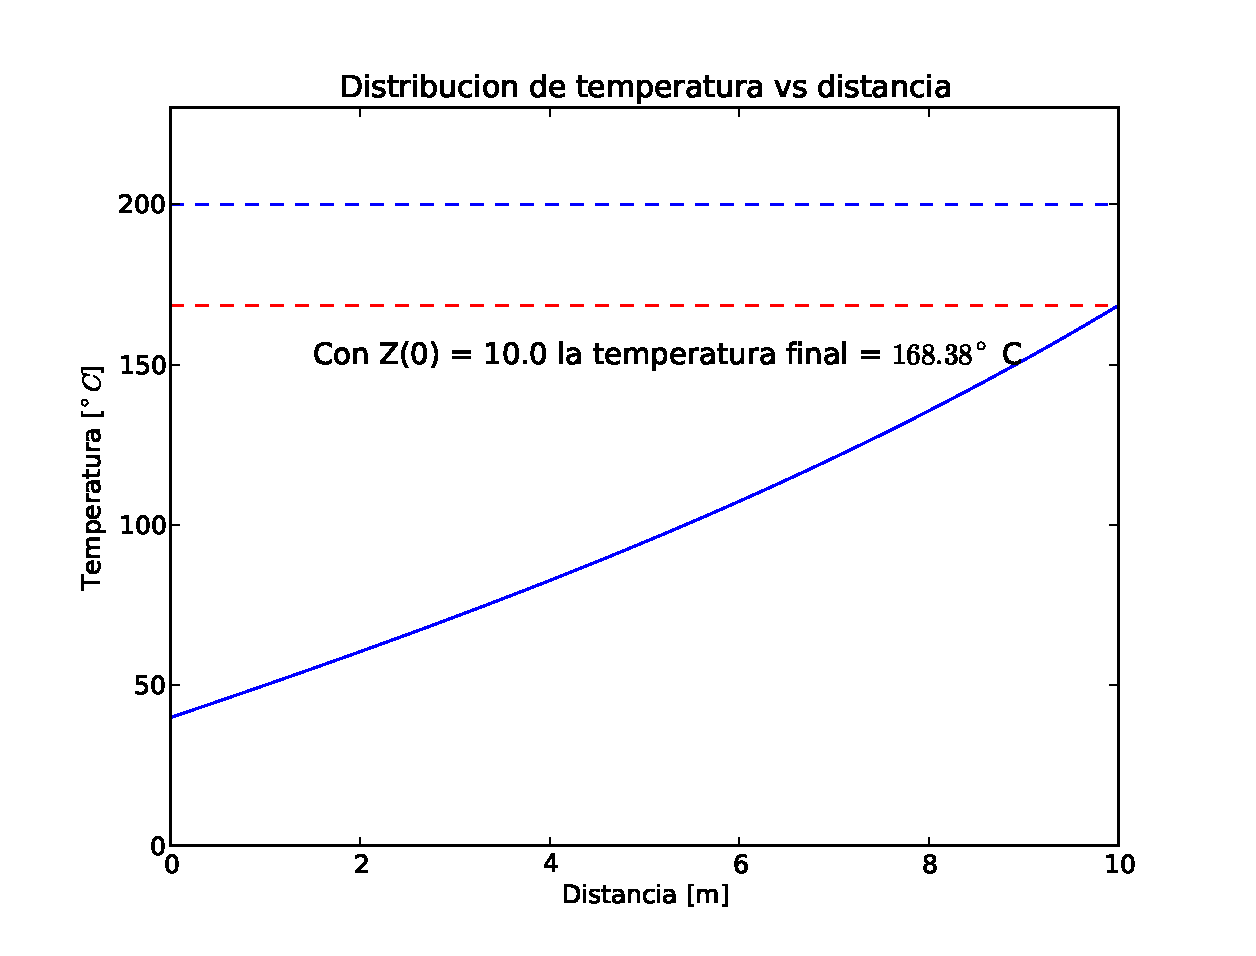
\includegraphics[scale=0.45]{MetDisparo01.eps} 
%\end{figure}
%\end{frame}
%\begin{frame}
%El resultado obtenido difiere de las condiciones de frontera $T(10)=200$, por lo que hacemos ahora otra suposición: $Z(0)=20$ y realizar de nuevo el cálculo.
%\end{frame}
%\begin{frame}
%\fontsize{12}{12}\selectfont
%\begin{center}
%\begin{tabular}{c | c | c}
%x & y[0] & y[1] \\ \hline 
%0.0000e+00 & 4.0000e+01 & 1.4000e+01 \\ \hline
%1.0000e+00 & 5.4123e+01 & 1.4270e+01 \\ \hline
%2.0000e+00 & 6.8588e+01 & 1.4684e+01 \\ \hline
%3.0000e+00 & 8.3540e+01 & 1.5244e+01 \\ \hline
%4.0000e+00 & 9.9127e+01 & 1.5957e+01 \\ \hline
%5.0000e+00 & 1.1551e+02 & 1.6829e+01 \\ \hline
%6.0000e+00 & 1.3284e+02 & 1.7870e+01 \\ \hline
%7.0000e+00 & 1.5131e+02 & 1.9090e+01 \\ \hline
%8.0000e+00 & 1.7108e+02 & 2.0500e+01 \\ \hline
%9.0000e+00 & 1.9237e+02 & 2.2116e+01 \\ \hline
%1.0000e+01 & 2.1539e+02 & 2.3954e+01
%\end{tabular}
%\end{center}
%\end{frame}
%\begin{frame}
%\frametitle{Gráficamente con $Z(0)= 14$}
%\begin{figure}
%	\centering
%	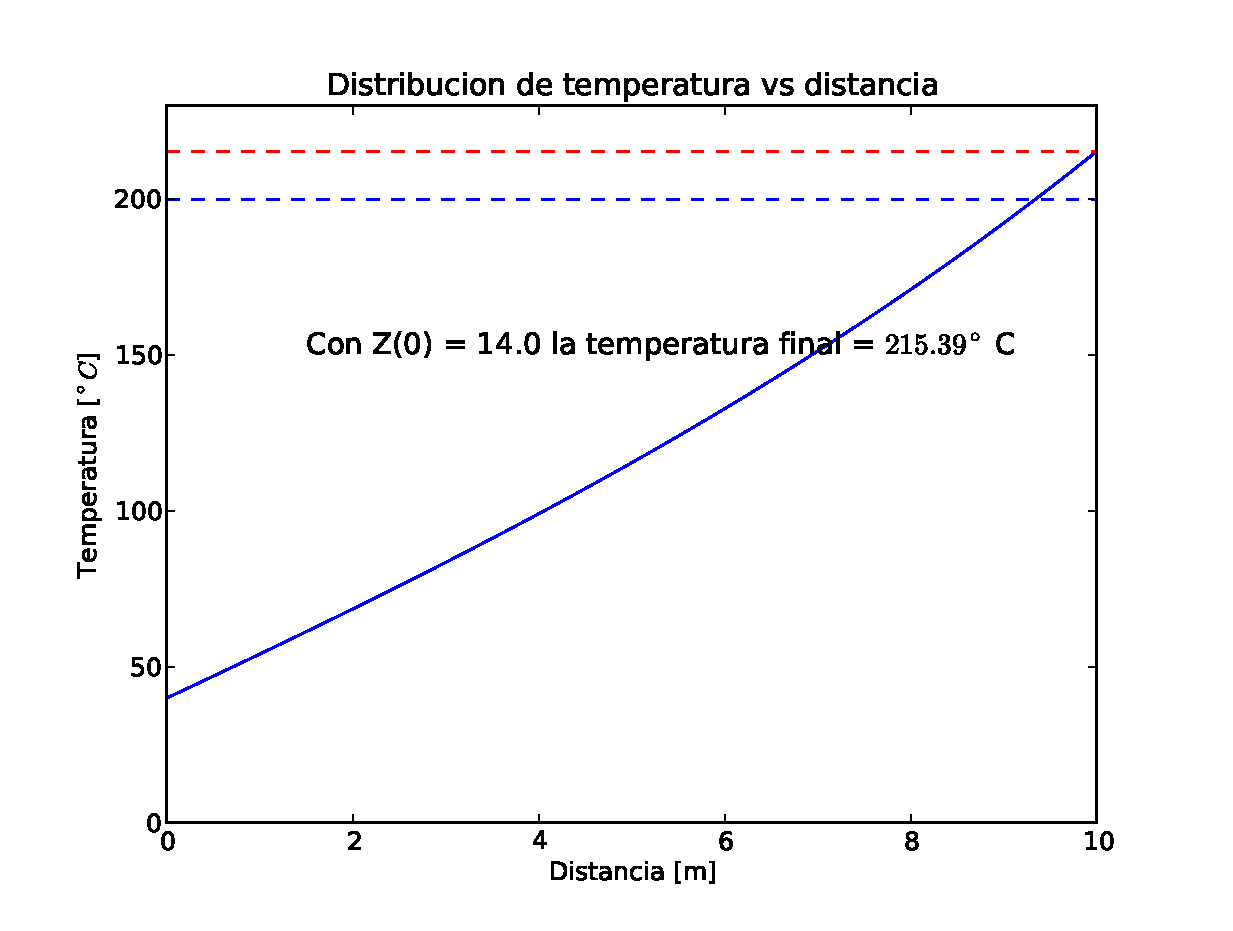
\includegraphics[scale=0.45]{MetDisparo02.eps} 
%\end{figure}
%\end{frame}
%\begin{frame}
%Ahora como la EDO original es lineal, los valores
%\[ \begin{matrix}
%Z(0) = 10 & T(10) = 168.38 \\
%Z(0) = 20 & T(10) = 215.39
%\end{matrix} \]
%están relacionados linealmente. Así, podemos usarlos para calcular el valor de $Z(0)$ que resulte para $T(10)=200$.
%\\
%\bigskip
%Podemos usar una fórmula de interpolación lineal
%\[ Z(0) =  10 + \dfrac{14-10}{215.39 - 168.37}(200-168.37) = 12.69 \]
%\end{frame}
%\begin{frame}
%\fontsize{12}{12}\selectfont
%\begin{center}
%\begin{tabular}{c | c | c}
%x & y[0] & y[1] \\ \hline 
%0.0000e+00 & 4.0000e+01 & 1.2690e+01 \\ \hline
%1.0000e+00 & 5.2811e+01 & 1.2954e+01 \\ \hline
%2.0000e+00 & 6.5951e+01 & 1.3347e+01 \\ \hline
%3.0000e+00 & 7.9550e+01 & 1.3874e+01 \\ \hline
%4.0000e+00 & 9.3746e+01 & 1.4540e+01 \\ \hline
%5.0000e+00 & 1.0868e+02 & 1.5352e+01 \\ \hline
%6.0000e+00 & 1.2450e+02 & 1.6317e+01 \\ \hline 
%7.0000e+00 & 1.4137e+02 & 1.7445e+01 \\ \hline
%8.0000e+00 & 1.5945e+02 & 1.8748e+01 \\ \hline
%9.0000e+00 & 1.7893e+02 & 2.0239e+01 \\ \hline
%1.0000e+01 & 1.9999e+02 & 2.1932e+01
%\end{tabular}
%\end{center}
%\end{frame}
%\begin{frame}
%\frametitle{Gráficamente con $Z(0)= 12.69$}
%\begin{figure}
%	\centering
%	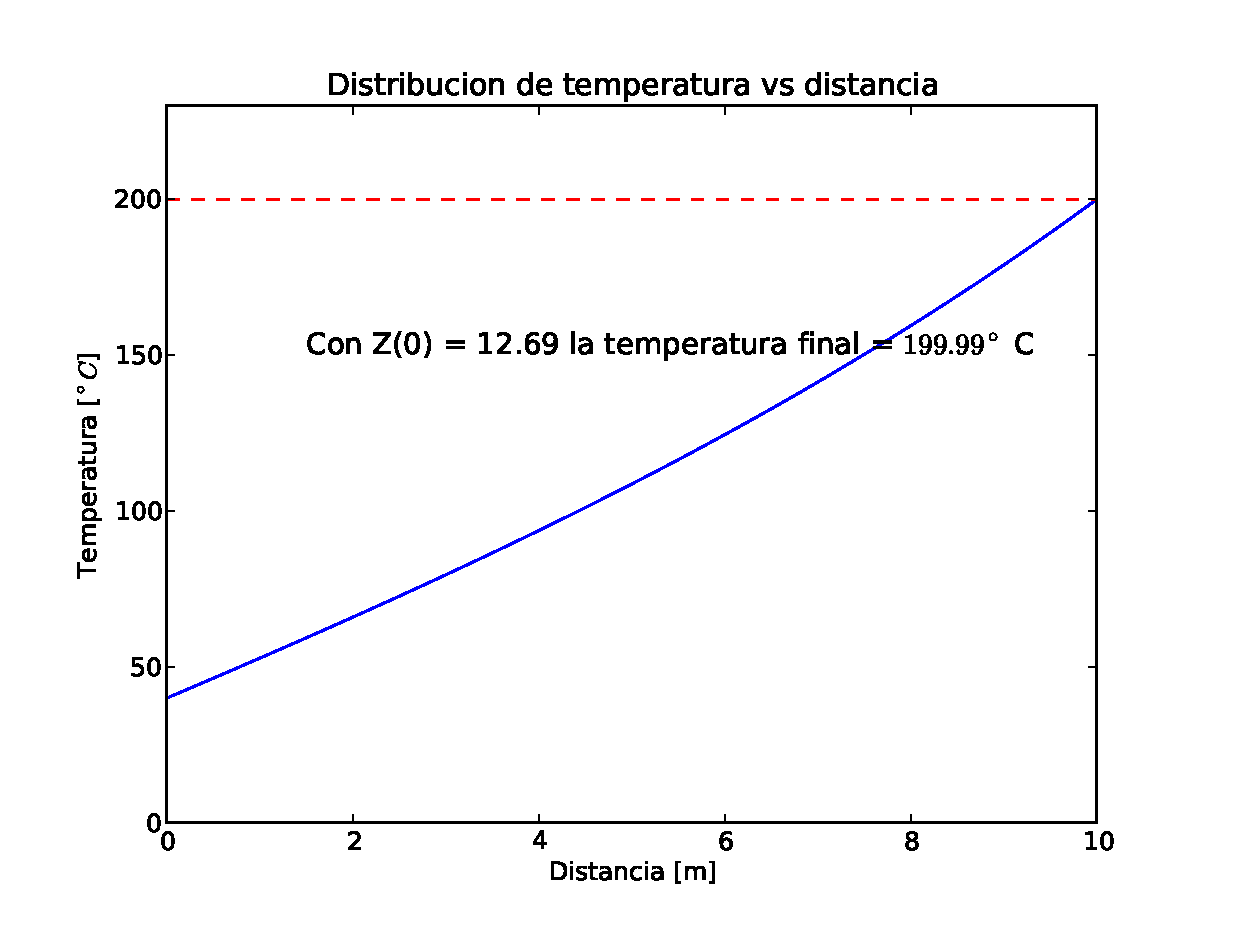
\includegraphics[scale=0.45]{MetDisparo03.eps} 
%\end{figure}
%\end{frame}
%\section{Problemas de Sturm-Liouville}
%\begin{frame}
%\frametitle{Problemas de Sturm-Liouville}
%Diversos problemas con condiciones en la frontera conducen (mediante el método de separación de variables) a la misma ecuación diferencial ordinaria
%\[ X''(x) + \lambda X(x) = 0, \hspace{1cm} (0 < x < L)\]
%con el valor propio $\lambda$, pero con distintas condiciones en los extremos:
%\begin{enumerate}
%\item $X(0) = X(L) = 0$ \hspace{1cm} Condición de Dirichlet.
%\item $X'(0) = X'(L) = 0$ \hspace{1cm} Condición de Neumann.
%\item $X(0) = X'(L) = 0$ \hspace{1cm} Condición mixta.
%\end{enumerate}
%según las condiciones de frontera.
%\end{frame}
%\begin{frame}
%Por ejemplo, en el problema de hallar la temperatura $u(x,t)$ de una varilla $0 \leq x \leq L$ con la temperatura inicial dada $u(x,0)=f(x)$.
%\\
%\bigskip
%Como problema con valores en la frontera, este problema es igual al problema de determinar la temperatura dentro de una lámina de gran tamaño que ocupe la región $0 \leq x \leq L$ en el espacio $xyz$.
%\end{frame}
%\begin{frame}
%Si su temperatura inicial sólo depende de $x$ y es independiente de $y$, $z$ (es decir, si $u(x,0)= f(x)$, entonces lo mismo será cierto de su temperatura $u=u(x,y)$ en el instante $t$. Sustituyendo
%\[u(x,t) = X(x)T(t)\]
%en la ecuación de calor
%\[ \dfrac{\partial u}{\partial t} = k \dfrac{\partial^{2} u}{\partial x^{2}}\]
%\end{frame}
%\begin{frame}
%Vemos que $X(x)$ satisface la condiciones en los extremos, si las caras $x=0$ y $x=L$ de la lámina se mantienen a temperatura cero.
%\\
%\bigskip
%Las condiciones de $X'(0) = X'(L) = 0$ si ambas caras están aisladas, y las de $X(0) = X'(L) = 0$, si una cara está aislada y la otra se mantiene a temperatura cero.
%\end{frame}
%\begin{frame}
%Pero si cada cara pierde calor hacia el medio ambiente (que se encuentra a temperatura cero) de acuerdo con la ley de enfriamiento de Newton, entonces las condiciones en los extremos asumen la forma
%\[h X(0) - X'(0) = 0 = h(X(L) + X'(L))\]
%donde $h$ es un coeficiente de transferencia de calor no negativo.
%\end{frame}
%\begin{frame}
%Al imponer diversas condiciones en los extremos sobre la solución del problema, obtenemos distintos problemas de valores propios, y por ello usamos distintos valores propios ${\lambda_{n}}$ y distintas funciones propioas $X_{n}(x)$ en la construcción de una solución formal en términos de una serie de potencias
%\[ u(x,t) = \sum c_{n} X_{n}(x) T_{n}(x)\]
%del problema con valores en la frontera. El paso final en esta construcción es la elección del coeficiente ${c_{n}}$ en la ecuación anterior de modo que
%\[u(x,0) = \sum c_{n} T_{n}(0)X_{n}(x)= f(x) \]
%\end{frame}
%\begin{frame}
%Por lo que necesitamos un desarrollo en términos de funciones propias de la función dada $f(x)$, en términos de las funciones propias del problema con valores en los extremos correspondientes.
%\end{frame}
%\begin{frame}
%\frametitle{Problemas de Sturm-Liouville}
%Para unificar y generalizar el método de separación de variables, es útil formular un tipo general de problema de valores propios que incluya como casos particulares a los ya mencionados.
%\\
%\bigskip
%La ecuación inicial, con $y$ en vez de $X$ como variable dependiente, se puede escribir como
%\[ \dfrac{d}{dx} \left[ p(x) \dfrac{dy}{dx} \right] - q(x) y + \lambda r(x) y = 0\]
%donde $p(x)=r(x) \equiv 1$ y $q(x) \equiv 0$
%\end{frame}
%\begin{frame}
%Podemos asegurar que casi cualquier ecuación diferencial lineal de segundo orden de la forma
%\[ A(x) y'' + B(x) y' + C(x) y + \lambda D(x) y = 0\]
%asume la forma indicada después de multiplicar por un factor adecuado.
%\end{frame}
%\begin{frame}
%\frametitle{Ejemplo}
%Si multiplicamos la ecuación paramétrica de Bessel de orden $n$
%\[ x^{2} y'' + xy' + (\lambda x^{2} - n^{2}) y = 0, \hspace{1cm} x>0\]
%por $1/x$, podemos escribir el resultado como
%\[ \dfrac{d}{dx} \left[ x \dfrac{dy}{dx} \right] - \dfrac{n^{2}}{x}y + \lambda x y = 0\]
%que tiene la forma S-L, con $p(x)=r(x)= x$ y $q(x) = n^{2}/x$
%\end{frame}
%\begin{frame}
%Imponiendo sobre las soluciones de la ecuación anterior, en un intervalo abierto acotado $(a,b)$ las siguientes condiciones -lineales- homogéneas en los extremos:
%\[ \begin{split}
%\alpha_{1} y(a) - \alpha_{2} y'(a) =& 0 \\
%\beta_{1} y(b) - \beta_{2} y'(b) =& 0
%\end{split} \]
%donde los coeficientes $\alpha_{1},\alpha_{2},\beta_{1},\beta_{2}$ son constantes.
%\end{frame}
%\begin{frame}
%Además de ser homogéneas, las condiciones están \textit{separadas}, en el sentido de que una de ellas implica los valores de $y(x)$ y $y'(x)$ en un extremo $x=a$, mientras que la otra implica los valores en el otro extremo $x=b$. Nótese que las condiciones $y(a)=y'(b)=0$ son d ela forma dada, con $\alpha_{1}=\beta_{2}=1$ y $\alpha_{2}=\beta_{1}=0$
%\end{frame}
%\subsection{Definición de un problema Sturm-Liouville}
%\begin{frame}
%\frametitle{Definición de un problema Sturm-Liouville}
%Un problema de Sturm-Liouville es un problema con valores en la frontera de la forma
%\[\dfrac{d}{dx} \left[ p(x) \dfrac{dy}{dx} \right] - q(x) y + \lambda r(x) y = 0, \hspace{1cm} a<x<b \]
%\[ \begin{split}
%\alpha_{1} y(a) - \alpha_{2} y'(a) =& 0 \\
%\beta_{1} y(b) - \beta_{2} y'(b) =& 0
%\end{split} \]
%donde tanto $\alpha_{1}$ y $\alpha_{2}$ como $\beta_{1}$ y $\beta_{2}$ son diferentes de cero. El parámetro $\lambda$ es el \textit{eingenvalor} cuyos posibles valores (constantes) se buscan.
%\end{frame}
%\begin{frame}
%\frametitle{Ejemplo}
%Se obtienen diferentes problemas de Sturm-Liouville complementando la ecuación diferencial
%\[ y'' + \lambda y = 0 \hspace{1cm} 0 < x < L\]
%con alguna de las diferentes condiciones de valores en la frontera homogéneas
%\begin{itemize}[<+->]
%\item $y(0) = y(L) = 0$, donde $\alpha_{1} = \beta_{1} = 1$ y $\alpha_{2} = \beta_{2} = 0$
%\item $y'(0) = y'(L) = 0$, donde $\alpha_{1} = \beta_{1} = 0$ y $\alpha_{2} = \beta_{2} = 1$
%\item $y(0) = y'(L) = 0$, donde $\alpha_{1} = \beta_{2} = 1$ y $\alpha_{2} = \beta_{1} = 0$
%\end{itemize}
%\end{frame}
%\begin{frame}
%Nótese que el problema S-L siempre tiene la solución trivial $y \equiv 0$, por consiguiente se buscan los valores de $\lambda$ (eingenvalores) para los cuales este problema tiene una solución real \textit{no trivial} (una eigenfunción) y cada eigenvalor cuenta con su eigenfunción asociada (o eigenfunciones).
%\\
%\bigskip
%Puede verse que cualquier constante (diferente de cero) múltiplo de una eigenfunción será también una eigenfunción.
%\end{frame}
%\subsection{Eigenvalores de Sturm-Liouville}
%\begin{frame}
%\frametitle{Eigenvalores de Sturm-Liouville}
%Supongamos que las funciones $p(x), p'(x),q(x)$ y $r(x)$ de la ecuación S-L son continuas en el intervalo $[a,b]$ y que tanto $p(x)>0$ como $r(x)>0$ en cada punto de $[a,b]$. De este modo los eigenvalores del problema de S-L, constituyen una sucesión creciente
%\[ \lambda_{1} < \lambda_{2} < \lambda_{3} < \ldots < \lambda_{n-1} < \lambda_{n} < \ldots\]
%de números reales, con
%\[ \lim_{n \rightarrow \infty} \lambda_{n} = + \infty\]
%Salvo por un factor constante, solo una eigenfunción $y_{n}(x)$ se asocia con cada eigenvalor $\lambda_{n}$.
%\end{frame}
%\begin{frame}
%Además, si $q(x) \geq 0$ en $[a,b]$ y los coeficientes $\alpha_{1},\alpha_{2},\beta_{1},\beta_{2}$ en la definición de S-L, son todos no negativos, entonces, los eigenvalores son todos no negativos.
%\\
%\bigskip
%Algunas veces el problema de S-L se llama \textbf{regular} si se satisface el resultado anterior, en caso contrario, es \textbf{singular}.
%\end{frame}
%\section{Una varilla delgada}
%\begin{frame}
%\frametitle{Una varilla delgada de metal}
%Sea una varilla delgada de metal con longitud $H$, sus extremos están conectados a distintas fuentes de calor:
%\begin{center}
%\begin{tikzpicture}[font=\small]
%\draw [fill=blue!20](0,0) rectangle node {$T_{L}$} (2,4);
%\draw (2,1.8) rectangle (3.5,2.2);
%\draw (4,1.8) rectangle (5.5,2.2);
%\draw [fill=blue!20] (5.5,0) rectangle node {$T_{R}$} (7.5,4);
%\draw [<->](2,1.3) -- node [midway, below] {x}(3.5,1.3);
%\draw [dashed] (3.5,2.2) -- (3.5,1.25);
%\draw [dashed] (4,2.2) -- (4,1.25);
%\draw [<-](4,1.3) -- node [midway, below] {dx}(4.6,1.3);
%\draw [<->] (2,0.1) -- node [midway, above] {H} (5.5,0.1);
%\draw (3.5,4) node {$T_{\infty}$};
%\end{tikzpicture}
%\end{center}
%\end{frame}
%\begin{frame}
%\fontsize{12}{12}\selectfont
%Si el calor sale de la superficie de la varilla únicamente por transferencia de calor, por medio de convección, la ecuación de temperatura es:
%\[ -A \dfrac{d}{dx} k(x) \dfrac{d}{dx} T(x) + h_{c} PT(x) = h_{c} PT_{\infty} + AS(x)\]
%donde
%\begin{itemize}
%\item $T(x)$ es la temperatura del punto que se encuentra a una distancia $x$ del extremo izquierdo.
%\item $A$ es el área constante de una sección transversal de la varilla.
%\item k es la conductividad térmica.
%\item P es el perímetro de la varilla.
%\item $h_{c}$ es el coeficiente de transferencia de calor por convección.
%\item $T_{\infty}$ es la temperatura neta del aire.
%\item S es la fuente de calor.
%\end{itemize}
%\end{frame}
%\begin{frame}
%Las condiciones de frontera son:
%\[ \begin{split} T(0) =& T_{L} \\
%T(H) =& T_{R}
%\end{split} \]
%Si $T^{0}$ se define como:
%\[ T^{0} = T - T_{\infty} \]
%\end{frame}
%\begin{frame}
%La ecuación de temperatura la podemos expresar como:
%\[ - \dfrac{d}{dx}k(x) \dfrac{d}{dx} T^{0}(x) + h_{c} \dfrac{P}{A} T^{0}(x) = S(x) \]
%El primer término representa la difusión del calor, el segundo es la pérdida de calor en el aire por medio de la convección y el lado derecho es la fuente de calor.
%\end{frame}
%\begin{frame}
%Otro ejemplo de una EDO con forma similar es la ecuación de difusión de neutrones dada por:
%\[ - \dfrac{d}{dx} D(x) \dfrac{d}{dx} \Psi (x) + \sum_{a} \Psi (x) = S(x) \]
%Donde $\Psi$ es el flujo de neutrones, $D$ es el coeficiente de difusión y $S$ es la fuente de neutrones.
%\\
%\bigskip
%El primer término indica la difusión de neutrones, el segundo la pérdida por absorción y el lado derecho es la fuente de neutrones.
%\end{frame}
%\begin{frame}
%Considerando en otros casos dentro de la física para problemas con difusión, si se expresa en términos de:
%\[- \dfrac{d}{dx} p(x) \dfrac{d}{dx} \phi (x) + q(x) \phi (x) = S(x)  \]
%siendo ésta, una ley de conservación de la difusión.
%\end{frame}
%\begin{frame}
%Integrando la ecuación anterior en el intervalo $[a,b]$, se obtiene que:
%\[ Z(b) - Z(a) + \int_{b}^{a} q(x) \phi (x) dx = \int_{b}^{a} S(x) dx \]
%donde
%\[ Z(x) = - p(x) \dfrac{d}{dx} \phi (x) \]
%Los términos primero y segundo de la primera ecuación aquí mostrada, son respectivamente, el flujo hacia adentro y el flujo hacia afuera de la propiedad representada por $\phi$, el tercer término es la pérdida total en $[a,b]$ y el lado derecho, es la fuente total en $[a,b]$.
%\end{frame}
%\subsection{Problemas con valores en la frontera para varillas y láminas}
%\begin{frame}
%\frametitle{Problemas con valores en la frontera para varillas y láminas}
%Consideremos una EDO de segundo orden con valores en la frontera
%\[ - \phi'' (x) + q \phi (x) = S(x), \hspace{1cm} 0< x < H \]
%con condiciones de frontera:
%\begin{itemize}
%\item $\phi'(0) = 0$, condición de frontera izquierda.
%\item $\phi'(H) = \phi'_{R}$, condición de frontera derecha
%\end{itemize}
%\end{frame}
%\begin{frame}
%Si dividimos el dominio en $N$ intervalos de igual longitud, se obtiene una retícula donde los intervalos miden $h = H/N$
%\begin{center}
%\begin{tikzpicture}[font=\small]
%\draw (0,1) node {$\phi'=0$};
%\draw (7,1) node {$\phi'=\phi_{R}$};
%\draw (-1.3,0) -- (8,0);
%\foreach \x in {-1,...,7}
%	\draw [fill=red!25](\x,0) circle (0.05);
%\draw (-1.3,-0.5) node {x=-h};
%\draw (0,-0.5) node {0};
%\draw (1,-0.5) node {h};
%\draw (2,-0.5) node {2h};
%\draw (3,-0.5) node {3h};
%\draw (7,-0.5) node {Nh=H};
%\draw (-1.3,-1) node {i=0};
%\draw (0,-1) node {1};
%\draw (1,-1) node {2};
%\draw (2,-1) node {3};
%\draw (3,-1) node {4};
%\draw (6,-1) node {N};
%\draw (7,-1) node {N=N+1};
%\end{tikzpicture}
%\end{center}
%\end{frame}
%\begin{frame}
%Usando una aproximación por diferencias centrales al primer término de la EDO de segundo orden, obtenemos la ecuación en diferencias para
%la $i$-ésima retícula:
%\[ \dfrac{(-\phi_{i-1} + 2 \phi_{i} - \phi_{i+1})}{h^{2}} + q \phi_{i} = S_{i} \]
%donde $\phi_{i}=\phi(x_{i})$, $S_{i}=S(x_{i})$ y $q$ es constante.
%\end{frame}
%\begin{frame}
%Al multiplicar por $h^{2}$
%\[ - \phi_{i-1} + (2-w) \phi_{i} - \phi_{i+1} = h^{2}S_{i} \]
%donde $w=qh^{2}$.
%\\
%\bigskip
%Esta ecuación se puede aplicar a todos los puntos de la retícula, excepto cuando $i = 1$ e $i = N+1$.
%\end{frame}
%\begin{frame}
%La condición de la frontera izquierda $\phi'(0) = 0$, es equivalente a una condición simétrica en la frontera llamada condición adiabática en la frontera en el caso de la transferencia de calor.
%\\
%\bigskip
%Si se considera un punto hipotético de la retícula $i = 0$ localizado en $x = -h$, la ecuación anterior en el caso $i = 1$ es:
%\[-\phi_{0} + (2+w)\phi_{1} - \phi_{2} = h^{2}S_{1} \]
%\end{frame}
%\begin{frame}
%En esta ecuación
%\[-\phi_{0} + (2+w)\phi_{1} - \phi_{2} = h^{2}S_{1} \]
%podemos hacer $\phi_{0} = \phi_{2}$ debido a la simetría. Dividiendo entre dos, obtenemos lo siguiente:
%\[ (1 + \dfrac{w}{2}) \phi_{1} - \phi_{2} = \dfrac{1}{2} h^{2}S_{1}\]
%como $\phi_{N+1}= \phi(H)=\phi_{R}$ en la frontera derecha, la ecuación con $i=N$ es:
%\[ -\phi_{N+1} + (2+w) \phi_{N} = h^{2}S_{N} + \phi_{R}\]
%\end{frame}
%\begin{frame}
%Ordenando los términos anteriores:
%%\fontsize{10}{10}\selectfont
%\[ \scriptsize{\begin{matrix}
%(1+\frac{w}{2})\phi_{1} & -\phi_{2}      &                &           &            & & = h^{2}\frac{S_{1}}{2} \\
%-\phi_{1}               & +(2+w)\phi_{2} & -\phi_{3}      &           &            & & = h^{2}S_{2} \\
%                        & \phi_{2}       & +(2+w)\phi_{3} & -\phi_{4} &            & & = h^{2}S_{3} \\
%                        &                &                &           &            & & \ldots \\
%                        &                &                &           &            & & \ldots \\
%                        &                &                &           &-\phi_{N+1} & +(2+w)\phi_{N} & = h^{2}S_{N}+\phi_{R} 
%\end{matrix}} \]
%\end{frame}
%\begin{frame}
%Que en forma matricial, resulta
%\fontsize{10}{10}\selectfont
%\[ \small{\begin{bmatrix}
%1+w/2 & -1 & 0 & 0 & 0 & 0 \\
%-1 & 2+w & -1 & 0 & 0 & 0 \\
%0 & -1 & 2+w & -1 & 0 & 0 \\
%0 & 0 & 0 + \ddots & -1 & 0 & 0 \\
%0 & 0 & 0 & 0 & -1 & 2+w
%\end{bmatrix} 
%\begin{bmatrix}
%\phi_{1} \\
%\phi_{2} \\
%\phi_{3} \\
%\ddots \\
%\phi_{N} \\
%\end{bmatrix} =
%\begin{bmatrix}
%h^{2}S_{1}/2 \\
%h^{2}S_{2} \\
%h^{2}S_{3} \\
%\ddots \\
%h^{2}S_{N}+\phi_{R} \\
%\end{bmatrix}}
%\]
%Todos los elementos de la matriz son cero, excepto los de las tres diagonales. Esta forma especial recibe el nombre de \emph{matriz tridiagonal}, y aparece muy a menudo en los métodos numéricos para problemas con valores en la frontera.
%\end{frame}

\end{document}